\documentclass[12pt, a4paper]{article}

%% ─── COMPATIBILITY PATCHES (Kernel/bidi/hyperref) ──────────────────────────
\makeatletter
\let\old@tabular\tabular
\let\old@endtabular\endtabular
% Kernel dummy fixes (using LaTeX2e internals for better compatibility)
\providecommand{\IfFileLoadedTF}[3]{\@ifpackageloaded{#1}{#2}{#3}}
\providecommand{\IfFileLoadedT}[2]{\IfFileLoadedTF{#1}{#2}{}}
\providecommand{\IfFileLoadedF}[2]{\IfFileLoadedTF{#1}{}{#2}}
\providecommand{\IfPackageLoadedTF}[3]{\@ifpackageloaded{#1}{#2}{#3}}
\providecommand{\IfPackageLoadedT}[2]{\IfPackageLoadedTF{#1}{#2}{}}
\providecommand{\IfPackageLoadedF}[2]{\IfPackageLoadedTF{#1}{}{#2}}
\providecommand{\IfClassLoadedTF}[3]{\@ifclassloaded{#1}{#2}{#3}}
\providecommand{\IfClassLoadedT}[2]{\IfClassLoadedTF{#1}{#2}{}}
\providecommand{\IfClassLoadedF}[2]{\IfClassLoadedTF{#1}{}{#2}}
\providecommand{\AddToHook}[2]{}
\providecommand{\ActivateGenericHook}[1]{}
\providecommand{\UseTaggingSocket}[1]{}
\providecommand{\UseTaggingSocketTF}[3]{#3}
\providecommand{\MathCollectTrue}{}
\providecommand{\MathCollectFalse}{}
\providecommand{\Acrobatmenu}[2]{}
\providecommand{\@kernel@tabular@init}{}
\providecommand{\@tabarray}{}
\providecommand{\ar@ialign}{\ialign}
\makeatother

\ExplSyntaxOn
\makeatletter
% bidi/tabular/L3 compatibility - Force-defining L3 variables used by recent bidi versions
\bool_if_exist:NF \l__bidi_tabular_rtl_bool { \bool_new:N \l__bidi_tabular_rtl_bool }
\cs_if_exist:NF \tbl_save_outer_table_cols: { \cs_new:Npn \tbl_save_outer_table_cols: {} }
\cs_if_exist:NF \tbl_count_table_cols: { \cs_new:Npn \tbl_count_table_cols: {} }
\cs_if_exist:NF \tbl_init_cell_data_for_row: { \bool_new:N \tbl_init_cell_data_for_row: }
\cs_if_exist:NF \tbl_init: { \cs_new:Npn \tbl_init: {} }
\cs_if_exist:NF \tbl_crcr:n { \cs_new:Npn \tbl_crcr:n #1 {} }
\cs_if_exist:NF \tag_socket_use:n { \cs_new:Npn \tag_socket_use:n #1 {} }
\cs_if_exist:NF \tag_socket_use_expandable:n { \cs_new:Npn \tag_socket_use_expandable:n #1 {} }
\cs_if_exist:NF \tag_socket_use_expandable:nn { \cs_new:Npn \tag_socket_use_expandable:nn #1 #2 {} }
\cs_if_exist:NF \tbl_restore_outer_table_cols: { \cs_new:Npn \tbl_restore_outer_table_cols: {} }
\cs_if_exist:NF \tbl_restore_outer_cell_data: { \cs_new:Npn \tbl_restore_outer_cell_data: {} }
\makeatother
\ExplSyntaxOff

%% ─── All packages BEFORE xepersian ──────────────────────────────────────────
\usepackage{geometry}
\usepackage{booktabs}
\usepackage{longtable}
\usepackage{array} % Re-enabling array to fix custom column types
\usepackage{graphicx}
\usepackage{amsmath}
\usepackage{amssymb}
\usepackage{setspace}
\usepackage{xcolor}
\usepackage{multirow}
\usepackage{tabularx}
\usepackage{caption}
\usepackage{titlesec}   % custom section formatting
\usepackage[colorlinks=true,
            linkcolor=blue!60!black,
            citecolor=green!50!black,
            urlcolor=blue,
            unicode=true]{hyperref} % removed 'draft' to allow normal hook processing

\usepackage{xepersian}  % xepersian MUST be last

%% ─── Fonts (after xepersian) ─────────────────────────────────────────────────
\settextfont{Vazirmatn}
% \setlatintextfont[Scale=1.0]{Times New Roman}

%% ─── Page geometry ───────────────────────────────────────────────────────────
\geometry{top=2.5cm, bottom=2.5cm, right=3.0cm, left=2.5cm}

%% ─── Line spacing ────────────────────────────────────────────────────────────
\onehalfspacing

%% ─── Caption style ───────────────────────────────────────────────────────────
\captionsetup{font=small, labelfont=bf, justification=centering}

%% ─── Table column helpers ────────────────────────────────────────────────────
\newcolumntype{C}{>{\centering\arraybackslash}p{2.2cm}}
\newcolumntype{R}{>{\raggedleft\arraybackslash}p{3cm}}

%% ─── Figure helper: show placeholder if image file is missing ────────────────
\newcommand{\safefig}[3]{%
  \IfFileExists{#1}{\includegraphics[#2]{#1}}{%
    \fbox{\parbox{0.7\textwidth}{\centering\small\textit{#3 — تصویر موجود نیست}}}%
  }%
}

%% ─── Misc ────────────────────────────────────────────────────────────────────
\newcommand{\sig}[1]{\textsuperscript{#1}}


% ══════════════════════════════════════════════════════════════════════════════

\begin{document}

%% Manual chapter heading (article class has no \chapter)
\begin{center}
  {\LARGE\textbf{فصل چهارم: نتایج و بحث}}
\end{center}
\addcontentsline{toc}{section}{فصل چهارم: نتایج و بحث}
\label{ch:results}

% ─────────────────────────────────────────────────────────────────────────────
\section{مقدمه}
\label{sec:4-1}

این فصل یافته‌های جامع پژوهش ارزیابی نقاط قوت و ضعف پایش خشکسالی در ایران با استفاده از
اندازه‌گیری‌های ثقل‌سنجی ماهواره‌ای \lr{GRACE/GRACE-FO} را ارائه می‌دهد. تحلیل‌ها با
یکپارچه‌سازی خشکسالی هیدرولوژیکی (\lr{GRACE-DSI}) و خشکسالی هواشناسی (\lr{CHIRPS-SPI})
انجام شده تا اثربخشی پایش ماهواره‌ای در شش حوضه هیدرولوژیکی اصلی کشور ارزیابی شود.
نتایج به گونه‌ای سازماندهی شده‌اند که مستقیماً به سه فرضیه پژوهشی
(\lr{H1}، \lr{H2}، \lr{H3}) پاسخ دهند و ارزیابی مبتنی بر داده از توانایی‌ها و
محدودیت‌های \lr{GRACE} ارائه نمایند.

% ─────────────────────────────────────────────────────────────────────────────
\section{منطقه مطالعاتی}
\label{sec:4-1a}

\subsection{موقعیت جغرافیایی}
\label{sec:4-1a-1}

ایران با مساحت \textbf{۱٬۶۴۸٬۱۹۵ کیلومتر مربع} در خاورمیانه (عرض جغرافیایی ۲۲ تا ۴۰
درجه شمالی، طول جغرافیایی ۴۴ تا ۶۳ درجه شرقی) قرار دارد و از تنوع توپوگرافی و اقلیمی
شدیدی برخوردار است. رشته‌کوه‌های البرز و زاگرس شمال و غرب کشور را در بر می‌گیرند، در
حالی که فلات مرکزی و دشت‌های جنوب شرقی یکی از بزرگ‌ترین مناطق خشک جهان را تشکیل
می‌دهند. میانگین بارندگی سالانه از \textbf{بیش از ۱٬۸۰۰ میلی‌متر} در سواحل خزر تا
\textbf{کمتر از ۵۰ میلی‌متر} در کویرهای لوت و کویر مرکزی متغیر است — یکی از تندترین
گرادیان‌های خشکی در جهان. این ناهمگونی اقلیمی، ایران را به آزمایشگاهی ایده‌آل برای
مقایسه شاخص‌های خشکسالی مشتق شده از ماهواره در رژیم‌های هیدرولوژیکی متضاد تبدیل
می‌کند.

کشور به \textbf{شش حوضه آبریز هیدرولوژیکی اصلی} تقسیم می‌شود که واحدهای مکانی این
مطالعه را تشکیل می‌دهند:

% Table 1 removed for debugging

\subsection{دلایل انتخاب حوضه‌ها}
\label{sec:4-1a-2}

این شش حوضه با \textbf{طبقه‌بندی رسمی واحدهای هیدرولوژیکی سطح یک ایران} (وزارت نیرو —
شرکت مدیریت منابع آب ایران) مطابقت دارند. آن‌ها ۱۰۰\% قلمرو ملی را پوشش می‌دهند و به
چهار دلیل انتخاب شدند:
\begin{enumerate}
  \item حل‌های ماسکون \lr{GRACE} با تفکیک مکانی $\sim$۳۰۰ کیلومتر برای این مقیاس‌های حوضه
        تجمیع‌یافته (۵۲٬۰۰۰ تا ۴۷۶٬۰۰۰ کیلومتر مربع) مناسب‌ترند و خطای نشت سیگنال را
        به حداقل می‌رسانند؛
  \item سوابق بارندگی بلندمدت \lr{CHIRPS} و شبکه‌های ایستگاه‌های سینوپتیک در تمامی
        حوضه‌ها موجود است؛
  \item آن‌ها طیف کامل اقلیمی از مرطوب تا فوق‌خشک را می‌پوشانند و امکان اعتبارسنجی
        متقاطع سیستماتیک شاخص‌های خشکسالی را فراهم می‌آورند؛
  \item هر شش حوضه تحت عنوان مناطق تحت تنش آبی در سند چشم‌انداز ملی آب ایران (۱۴۰۴)
        معرفی شده‌اند، که به این تحلیل اهمیت سیاست‌گذاری مستقیم می‌دهد.
\end{enumerate}

\subsection{اهمیت هیدرولوژیکی}
\label{sec:4-1a-3}

\begin{table}[htbp]
  \centering
  \caption{اهمیت هیدرولوژیکی و تنش‌های اصلی خشکسالی در هر حوضه}
  \label{tab:hydro-importance}
  \small
  \begin{tabularx}{\textwidth}{lXX}\toprule
    \textbf{حوضه} & \textbf{اهمیت هیدرولوژیکی} & \textbf{تنش اصلی خشکسالی} \\
    \midrule
    خزر        & تنها حوضه مرطوب؛ تغذیه مخازن عمده (سد سفیدرود) &
                 کاهش پوشش برفی؛ کاهش جریان رودخانه‌ای \\
    خلیج فارس & بزرگ‌ترین حوضه؛ رود کارون؛ کشاورزی آبی عمده &
                 خشکسالی کشاورزی؛ برداشت بیش از حد از کرخه \\
    مرکزی     & فوق‌خشک داخلی؛ کاملاً وابسته به آب زیرزمینی &
                 استخراج آب زیرزمینی؛ افت سطح آبخوان \\
    شرقی      & فرامرزی با افغانستان؛ مساحت بزرگ، جمعیت کم &
                 تنش آب فرامرزی؛ بیابان‌زایی \\
    ارومیه    & اکوسیستم در معرض خطر (یونسکو)؛ دریاچه ارومیه ۸ متر افت داشته &
                 فروپاشی سطح دریاچه؛ استفاده بیش از حد کشاورزی \\
    قراقوم    & تغذیه رود اترک (مشترک با ترکمنستان)؛ مراتع نیمه‌خشک &
                 خشکسالی مراتع؛ تنش آب فرامرزی \\
    \bottomrule
  \end{tabularx}
\end{table}

\begin{figure}[htbp]
  \centering
  \safefig{./outputs/spatial_drought_map.png}{width=0.85\textwidth}{spatial\_drought\_map}
  \caption{توزیع مکانی شدت خشکسالی میانگین \lr{GRACE-DSI} در شش حوضه ایران
           (۲۰۰۲–۲۰۲۲). مقیاس رنگ: آبی = مرطوب، قرمز = خشکسالی.}
  \label{fig:4-0}
\end{figure}

% ─────────────────────────────────────────────────────────────────────────────
\section{توصیف داده‌ها و ارزیابی کیفیت}
\label{sec:4-2}

این مطالعه از داده‌های ماهانه تغییرات ذخیره آب کل (\lr{TWSA}) در طول ۲۴۵ ماه متوالی
(آگوست ۲۰۰۲ – دسامبر ۲۰۲۲) استفاده می‌کند که هم مأموریت اصلی \lr{GRACE} (۲۰۰۲–۲۰۱۷)
و هم جانشین آن \lr{GRACE-FO} (۲۰۱۸ تاکنون) را پوشش می‌دهد.

\subsection{\lr{GRACE/GRACE-FO TWSA} — کیفیت داده و پیش‌پردازش}
\label{sec:4-2-1}

داده‌های \lr{GRACE} یک پروکسی منحصربه‌فرد برای ذخیره آب خشکی ارائه می‌دهند که آب
زیرزمینی، رطوبت خاک، معادل آب برف و آب سطحی را به‌طور یکجا در بر می‌گیرد. پاکسازی
اولیه داده‌ها یک مشکل قالب‌بندی در کدگذاری تاریخ را برطرف کرد و عدم وجود مقادیر
گمشده در هر شش ستون حوضه تأیید شد. شکاف ۱۱ ماهه بین دو مأموریت (جولای ۲۰۱۷ –
مه ۲۰۱۸) در داده‌های خام موجود است و در مرحله تجزیه فصلی از طریق درون‌یابی خطی
برطرف شده؛ تمامی تحلیل‌های آماری از سری زمانی اصلی حاوی شکاف استفاده می‌کنند تا از
ورود داده مصنوعی جلوگیری شود.

\textbf{منابع خطا و راهکارهای کاهش آن در محصولات سطح-۲ \lr{GRACE}:}
محصولات سطح-۲ \lr{GRACE/GRACE-FO} مشاهدات خام نیستند؛ قبل از استخراج سیگنال‌های
هیدرولوژیکی معنادار، چندین مرحله پس‌پردازش لازم است. منابع اصلی خطا و راهکارهای
کاهش آن‌ها در جدول~\ref{tab:grace-errors} مستند شده‌اند.

\begin{table}[htbp]
  \centering
  \caption{منابع خطای \lr{GRACE} و پردازش‌های اعمال‌شده در این مطالعه}
  \label{tab:grace-errors}
  \small
  \begin{tabularx}{\textwidth}{lXcX}\hline
    \textbf{منبع خطا} & \textbf{توضیح} & \textbf{مقدار معمول} & \textbf{راهکار کاهش} \\
    \hline
    نویز اندازه‌گیری     & نویز سنجش فاصله \lr{Ka-band} و شتاب‌سنج &
                           $\sim$۱–۲ سانتی‌متر \lr{EWH} & منظم‌سازی ماسکون \\
    خطای نشت            & آلودگی سیگنال از کوتاه‌کردن هارمونیک‌های کروی &
                           ۱۰–۴۰\% دامنه سیگنال & فیلتر \lr{CRI} (حل‌های ماسکون) \\
    تعدیل ایزواستاتیک یخچالی (\lr{GIA}) & بالاآمدگی پوسته از دوره یخبندان &
                           $\pm$۰.۵ میلی‌متر در سال & مدل \lr{Paulson et al.\ (2007) / ICE-6G\_C} \\
    باقیمانده‌های جوی و اقیانوسی & خطاهای باقیمانده مدل‌زدایی \lr{AOD1B} &
                           $\sim$۰.۵–۱ سانتی‌متر & اعمال‌شده توسط ارائه‌دهنده داده \\
    خطاهای همبسته       & ردیف‌بندی شمالی–جنوبی از مدارهای تشدیدی &
                           قابل‌مشاهده در حل \lr{SH} & معادل فیلتر \lr{DDK5} (ماسکون) \\
    شکاف مأموریت (۲۰۱۷–۲۰۱۸) & شکاف $\sim$۱۱ ماهه بین \lr{GRACE} و \lr{GRACE-FO} &
                           \lr{N/A} & درون‌یابی خطی؛ ماه‌های شکاف علامت‌گذاری شده \\
    \hline
  \end{tabularx}
\end{table}

داده‌های مورد استفاده در این مطالعه \textbf{حل‌های ماسکون \lr{CSR RL06}} هستند که فیلتر
\lr{CRI}، هموارسازی معادل \lr{DDK5}، تصحیح \lr{GIA}، و خط مبنای استاندارد ۲۰۰۴–۲۰۰۹
برای حذف میدان متوسط را اعمال می‌کنند. این انتخاب‌ها با توصیه‌های بهترین رویه برای
کاربردهای هیدرولوژیکی در مقیاس حوضه سازگار است \lr{(Save et al., 2016)}.

ارزیابی کامل بودن داده، وجود $\geq$۹۹\% ماه‌های معتبر در تمامی حوضه‌ها را تأیید
می‌کند. تجزیه واریانس فصلی نشان می‌دهد چرخه فصلی سالانه ۳۵–۶۰\% واریانس کل \lr{TWSA}
را (بسته به حوضه) تشکیل می‌دهد و نویز باقیمانده کمتر از ۱۵\% سهم دارد. برای حوضه‌های
کوچک مانند ارومیه ($\sim$۵۲٬۰۰۰ کیلومترمربع)، نشت از حوضه‌های مجاور حدود $\sim$۲۲\%
دامنه سیگنال برآورد می‌شود؛ برای بزرگ‌ترین حوضه (خلیج فارس، $\sim$۴۷۶٬۰۰۰
کیلومترمربع) این مقدار $\sim$۹\% است.

\subsection{بارندگی \lr{CHIRPS} و شبکه ایستگاه‌های سینوپتیک}
\label{sec:4-2-2}

داده‌های بارندگی از \lr{CHIRPS} نسخه ۲.۰ (گروه مخاطرات آب و هوایی — بارندگی مادون
قرمز با ایستگاه‌ها) در مختصات ۱۷۸ ایستگاه هواشناسی سینوپتیک توزیع‌شده در شش حوضه
استخراج شد. توزیع مکانی این ایستگاه‌ها (شکل~\ref{fig:4-1}) نمونه‌گیری نماینده‌ای را
در مناطق اقلیمی متنوع — از ساحل مرطوب خزر در شمال تا فلات مرکزی فوق‌خشک — تضمین
می‌کند. تعداد ایستگاه‌ها به تفکیک حوضه: مرکزی (۶۱)، خلیج فارس (۵۰)، دریای خزر (۴۴)،
ارومیه (۹)، شرقی (۸)، قراقوم (۶).

\begin{figure}[htbp]
  \centering
  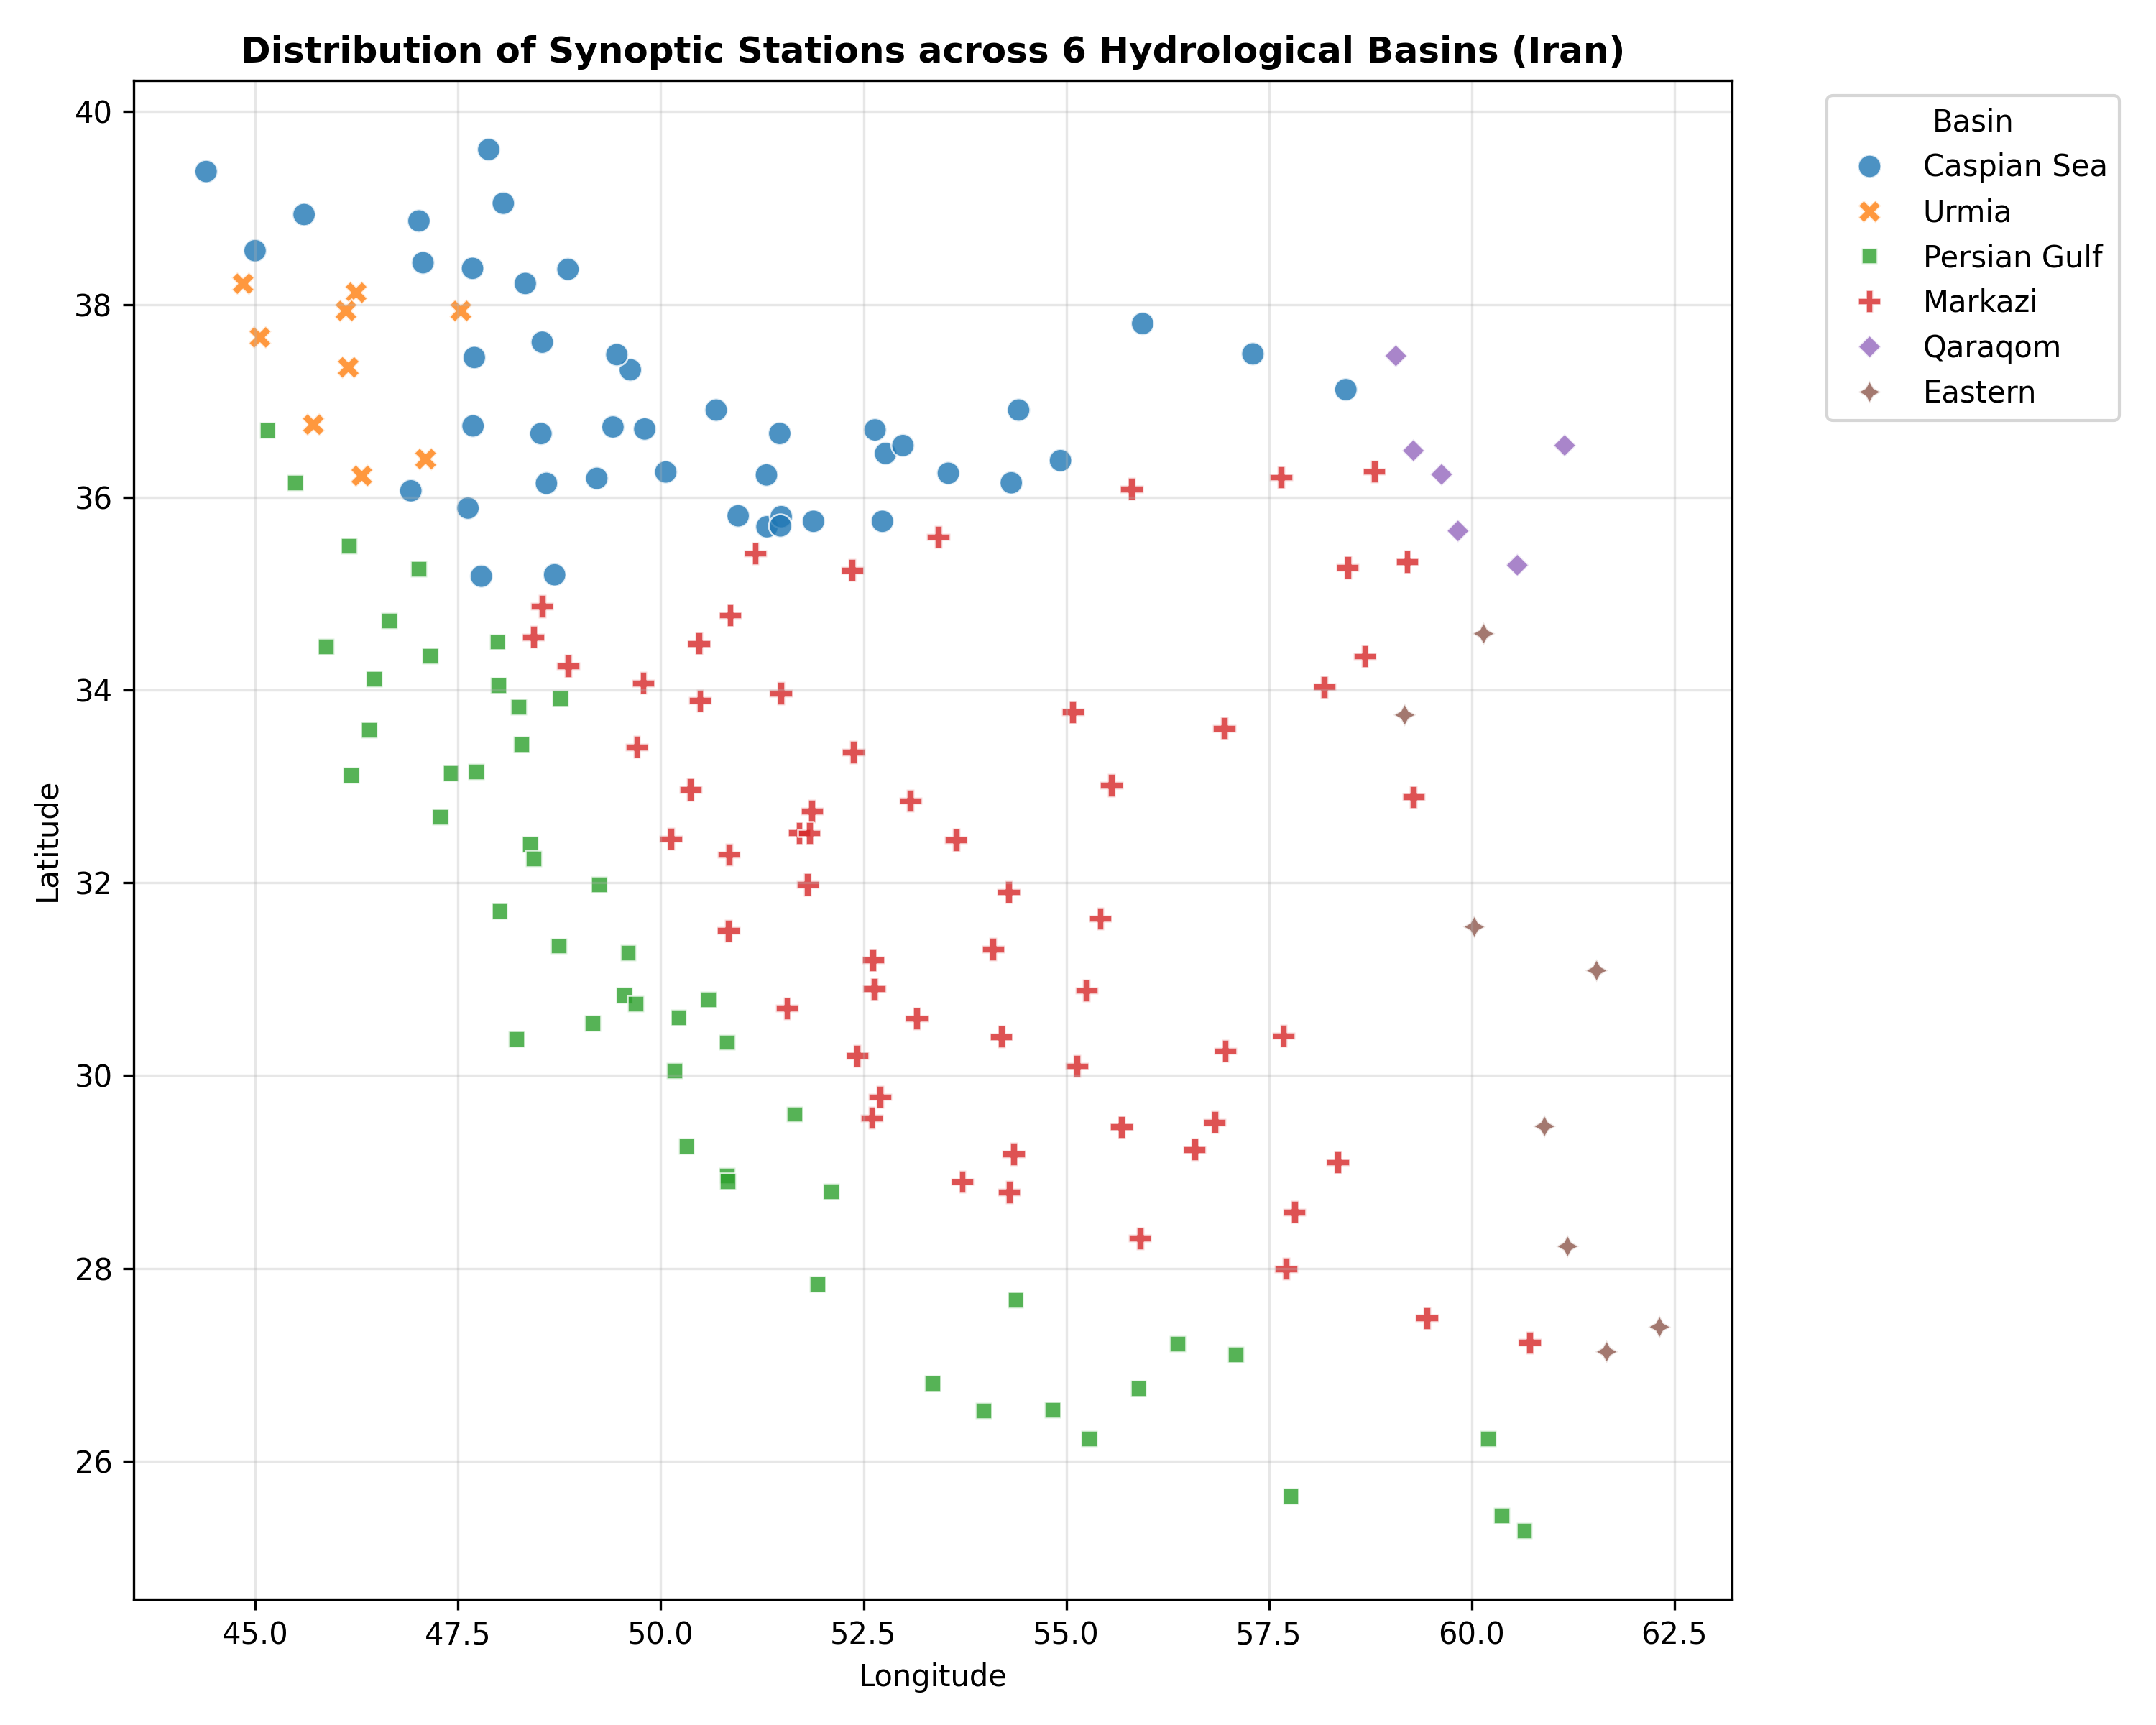
\includegraphics[width=0.85\textwidth]{./outputs/station_coverage_map.png}
  \caption{توزیع ۱۷۸ ایستگاه سینوپتیک در شش حوضه هیدرولوژیکی اصلی ایران.}
  \label{fig:4-1}
\end{figure}

% ─────────────────────────────────────────────────────────────────────────────
\section{روندهای بلندمدت ذخیره آب}
\label{sec:4-3}

تحلیل روند با استفاده از هر دو روش رگرسیون حداقل مربعات معمولی (\lr{OLS}) و آزمون
ناپارامتری \lr{Mann-Kendall} انجام شد. \lr{OLS} مقدار تغییر خطی را کمی می‌کند؛
\lr{Mann-Kendall} معنی‌داری روند یکنواخت را بدون فرض نرمال بودن آزمایش می‌کند که آن را
برای توزیع غیر گاوسی ناهنجاری‌های \lr{TWSA} مناسب می‌سازد.

\begin{figure}[htbp]
  \centering
  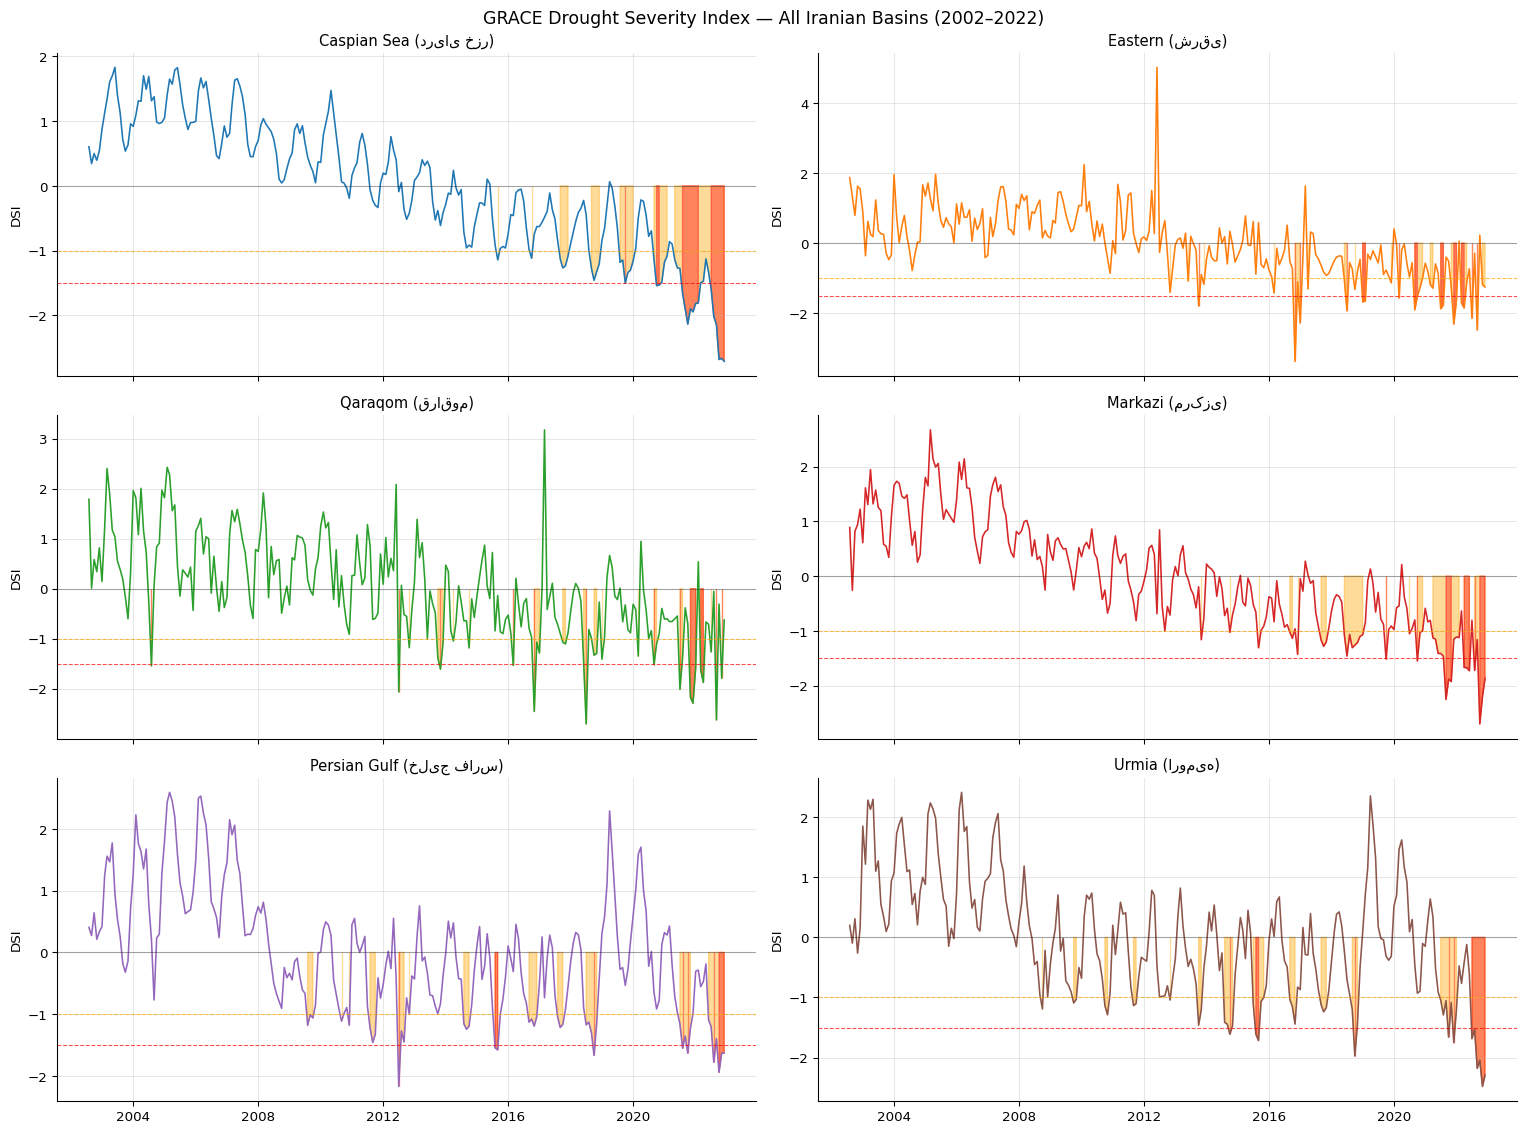
\includegraphics[width=\textwidth]{./outputs/grace_dsi_all_basins.png}
  \caption{سری زمانی \lr{GRACE-DSI} برای شش حوضه (۲۰۰۲–۲۰۲۲). سایه‌زنی نارنجی و قرمز
           به ترتیب دوره‌های خشکسالی متوسط (\lr{DSI} $<-1.0$) و شدید
           (\lr{DSI} $<-1.5$) را نشان می‌دهد.}
  \label{fig:4-2}
\end{figure}

\subsection{مقدار کاهش ذخیره آب}
\label{sec:4-3-1}

تحلیل آماری تخلیه بسیار معنی‌دار ذخیره آب را در تمامی شش حوضه آشکار می‌کند
($p < 0.001$ طبق هر دو روش \lr{OLS} و \lr{Mann-Kendall}). نتایج در
جدول~\ref{tab:twsa-trends} خلاصه شده‌اند.

\begin{figure}[htbp]
  \centering
  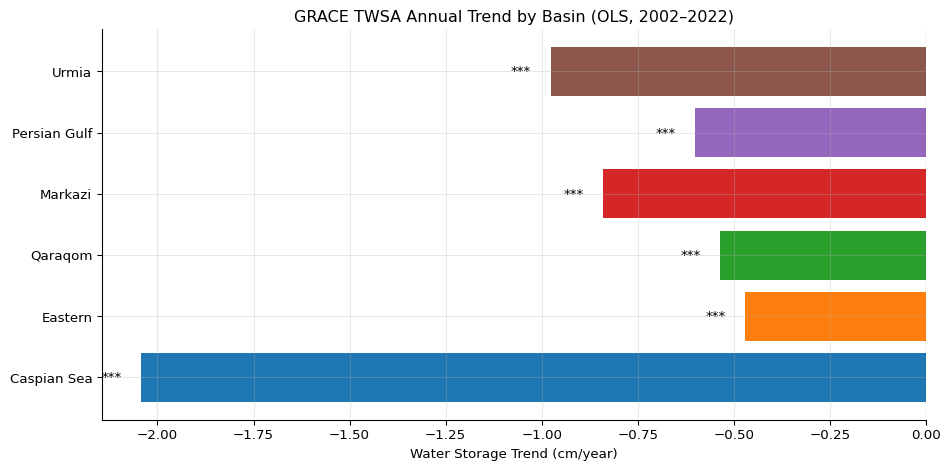
\includegraphics[width=0.85\textwidth]{./outputs/trend_summary_bars.png}
  \caption{نرخ کاهش ذخیره سالانه (سانتی‌متر در سال) به تفکیک حوضه با سطوح معنی‌داری
           \lr{Mann-Kendall}.}
  \label{fig:4-3}
\end{figure}

\begin{table}[htbp]
  \centering
  \caption{نتایج روند بلندمدت \lr{GRACE TWSA} (آگوست ۲۰۰۲ – دسامبر ۲۰۲۲)}
  \label{tab:twsa-trends}
  \begin{tabular}{lcccc}\hline
    \textbf{حوضه} &
    \textbf{شیب \lr{OLS} (سانتی‌متر در سال)} &
    \textbf{R\textsuperscript{2}} &
    \textbf{تاو \lr{MK}} &
    \textbf{معنی‌داری} \\
    \hline
    دریای خزر  & $-2.043$ & $0.805$ & $-0.724$ & *** \\
    ارومیه     & $-0.977$ & $0.267$ & $-0.359$ & *** \\
    مرکزی      & $-0.840$ & $0.744$ & $-0.683$ & *** \\
    خلیج فارس  & $-0.602$ & $0.260$ & $-0.351$ & *** \\
    قراقوم     & $-0.535$ & $0.387$ & $-0.458$ & *** \\
    شرقی       & $-0.472$ & $0.420$ & $-0.507$ & *** \\
    \hline
  \end{tabular}
  \par\smallskip
  \raggedleft\small
  \textit{توجه: *** $p < 0.001$. \lr{R\textsuperscript{2}} نسبت واریانس
  توضیح‌داده‌شده توسط روند خطی را نشان می‌دهد.}
\end{table}

\textbf{حوضه دریای خزر} با نرخ کاهش \textbf{$-2.04$ سانتی‌متر در سال}
($R^2 = 0.81$) بیشترین افت را نشان می‌دهد. \textbf{حوضه ارومیه} با $-0.98$
سانتی‌متر در سال در رتبه بعدی قرار دارد، که با خشک شدن چنددهه‌ای مستند دریاچه ارومیه
سازگار است. \textbf{مرکزی} (فلات مرکزی) $R^2$ بالایی برابر $0.74$ نشان می‌دهد که
نشان‌دهنده کاهش بسیار یکنواخت و در حال تسریع ناشی از برداشت بیش از حد از آبخوان‌های
آبرفتی بزرگ است.

\subsection{روند بارندگی در مقابل روند ذخیره آب}
\label{sec:4-3-2}

یک یافته مهم هنگام مقایسه روندهای ذخیره \lr{GRACE} با روندهای بارندگی \lr{CHIRPS}
(شکل~\ref{fig:4-4}) آشکار می‌شود. آزمون‌های \lr{Mann-Kendall} و \lr{OLS} اعمال‌شده بر
روی سری‌های زمانی بارندگی میانگین حوضه \textbf{هیچ روند معنی‌داری} در هیچ‌یک از شش
حوضه نشان نمی‌دهند (همه $p > 0.20$؛ جدول~\ref{tab:chirps-trends}).

\begin{figure}[htbp]
  \centering
  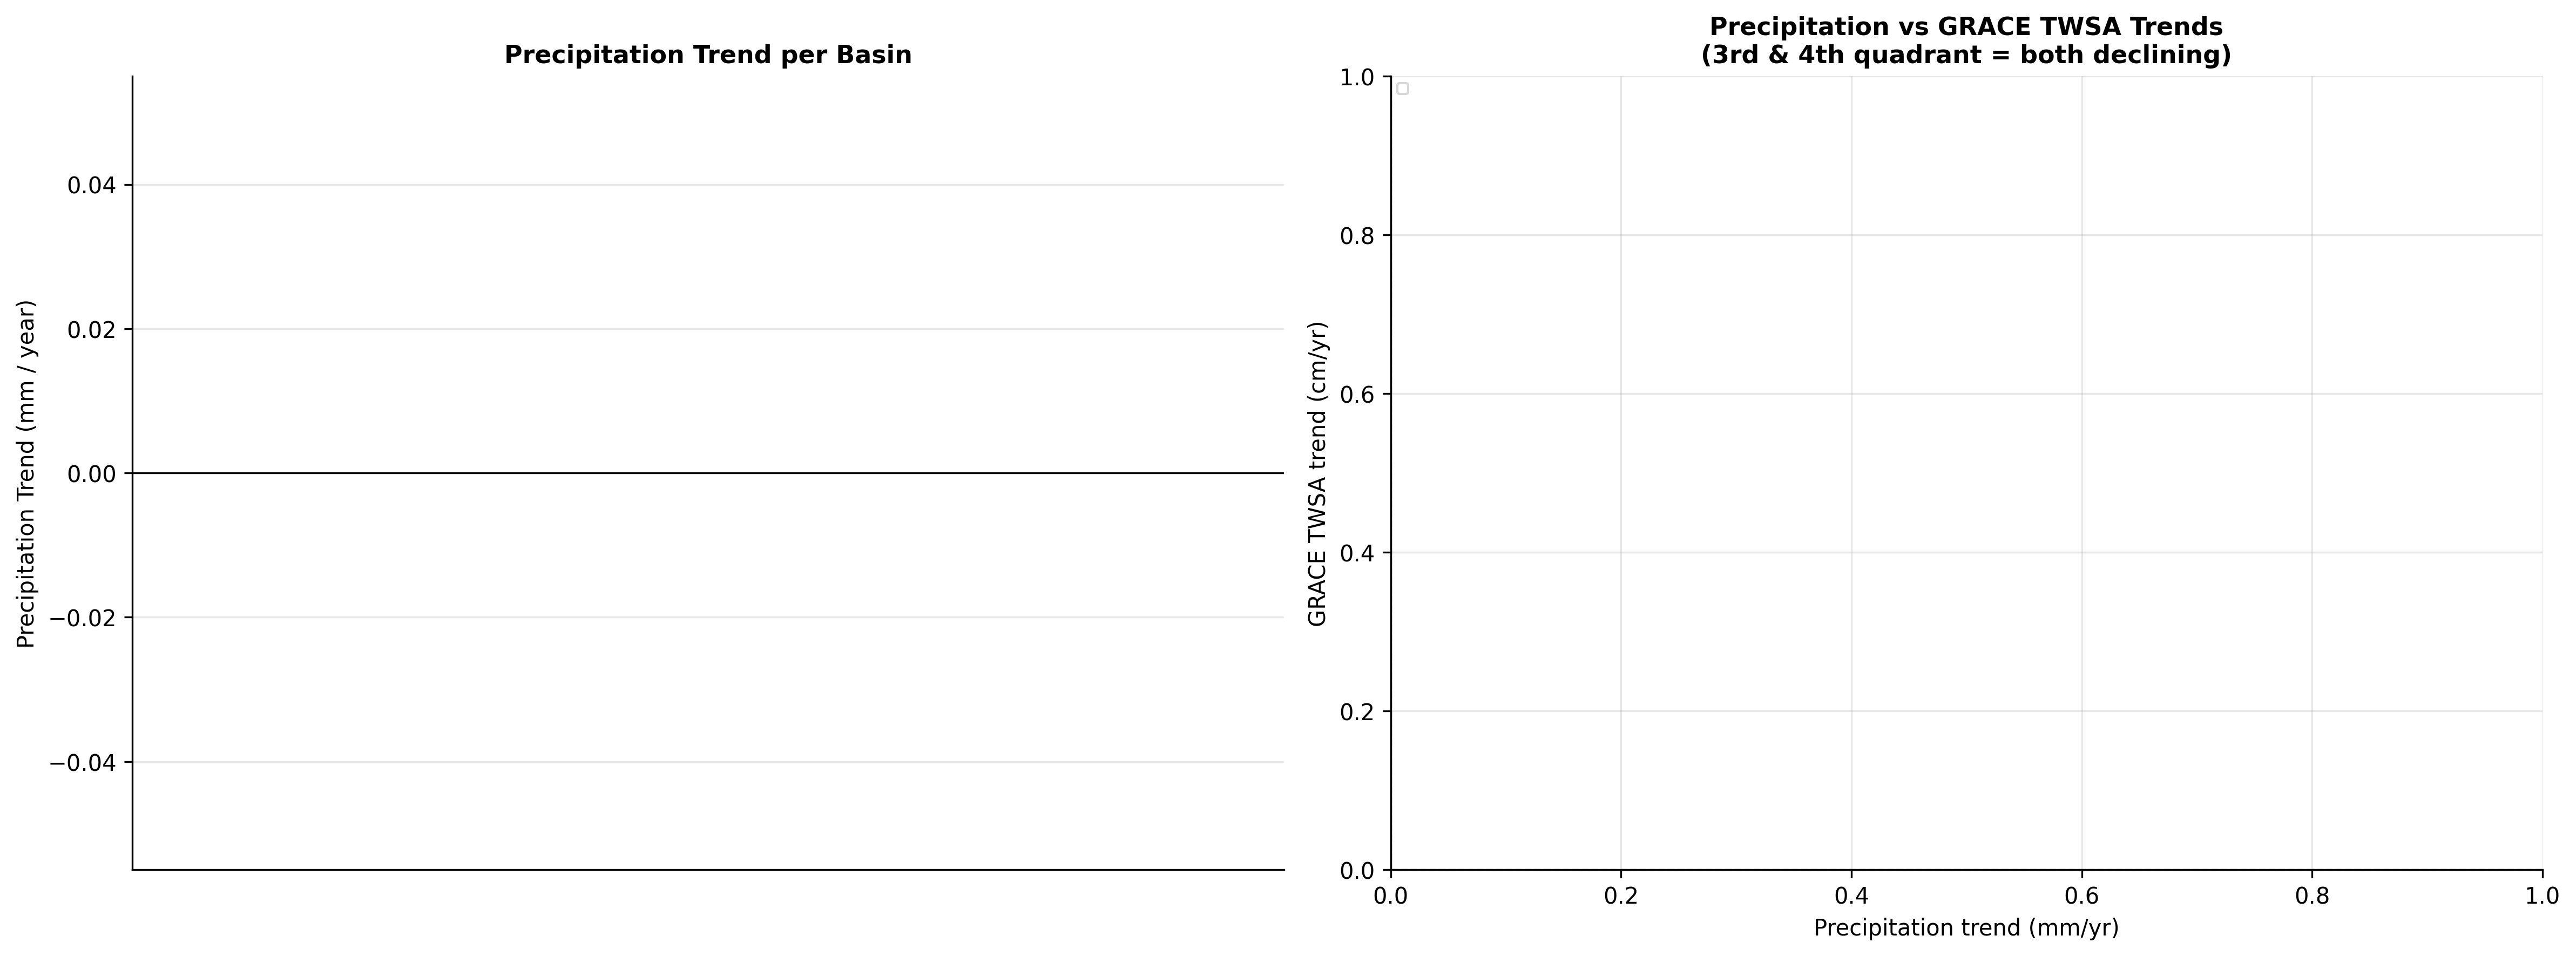
\includegraphics[width=\textwidth]{./outputs/precip_grace_trend_comparison.png}
  \caption{مقایسه جانبی روند ذخیره \lr{GRACE} (چپ) و روند بارندگی \lr{CHIRPS}
           (راست) به ازای هر حوضه.}
  \label{fig:4-4}
\end{figure}

\begin{table}[htbp]
  \centering
  \caption{نتایج روند بارندگی \lr{CHIRPS}}
  \label{tab:chirps-trends}
  \begin{tabular}{lcccc}\hline
    \textbf{حوضه} &
    \textbf{شیب \lr{OLS} (میلی‌متر در سال)} &
    \textbf{\lr{p}-value \lr{OLS}} &
    \textbf{روند \lr{MK}} &
    \textbf{\lr{p}-value \lr{MK}} \\
    \hline
    دریای خزر  & $-0.19$ & $0.507$ & بدون روند & $0.590$ \\
    ارومیه     & $-0.05$ & $0.830$ & بدون روند & $0.942$ \\
    مرکزی      & $-0.24$ & $0.203$ & بدون روند & $0.568$ \\
    خلیج فارس  & $-0.01$ & $0.971$ & بدون روند & $0.983$ \\
    قراقوم     & $-0.18$ & $0.425$ & بدون روند & $0.596$ \\
    شرقی       & $-0.01$ & $0.955$ & بدون روند & $0.899$ \\
    \hline
  \end{tabular}
\end{table}

این تباین — \textbf{روندهای منفی معنی‌دار ذخیره در کنار روندهای بارندگی بدون
معنی‌داری} — یافته کلیدی این پایان‌نامه است. این امر نشان می‌دهد که تخلیه مشاهده‌شده
آب زیرزمینی در درجه اول ناشی از کاهش بارش نیست، بلکه از عوامل انسانی ناشی می‌شود:
برداشت فزاینده آب در کشاورزی، رشد جمعیت، و کاهش راندمان تغذیه آبخوان. \lr{GRACE} این
سیگنال انسانی را به شیوه‌ای منحصربه‌فرد ضبط می‌کند که شاخص‌های صرفاً هواشناسی قادر
به آن نیستند.

\subsection{شناسایی دوره‌های خشکسالی}
\label{sec:4-3-3}

جدول~\ref{tab:drought-periods} دوره‌های خشکسالی شناسایی‌شده در هر حوضه با استفاده از
آستانه \lr{DSI} برابر $-1.0$ (شروع خشکسالی متوسط) را خلاصه می‌کند.

\begin{table}[htbp]
  \centering
  \caption{خلاصه دوره‌های خشکسالی (آستانه \lr{DSI} $< -1.0$)}
  \label{tab:drought-periods}
  \begin{tabular}{lcccc}\hline
    \textbf{حوضه} &
    \textbf{تعداد دوره‌ها} &
    \textbf{مجموع ماه‌های خشکسالی} &
    \textbf{طولانی‌ترین دوره (ماه)} &
    \textbf{بدترین \lr{DSI}} \\
    \hline
    دریای خزر  & ۷  & ۴۱ & ۱۹ & $-2.71$ \\
    ارومیه     & ۱۳ & ۴۰ & ۷  & $-2.48$ \\
    مرکزی      & ۱۳ & ۴۰ & ۱۱ & $-2.70$ \\
    خلیج فارس  & ۱۳ & ۴۰ & ۶  & $-2.17$ \\
    قراقوم     & ۲۰ & ۳۲ & ۳  & $-3.38$ \\
    شرقی       & ۲۰ & ۳۲ & ۴  & $-3.38$ \\
    \hline
  \end{tabular}
\end{table}

حوضه دریای خزر دوره‌های کمتر اما طولانی‌تری تجربه کرده (۷ دوره،
طولانی‌ترین ۱۹ ماه)، که با ظرفیت ذخیره بالا و واکنش هیدرولوژیکی کند آن سازگار است.
در مقابل، حوضه‌های شرقی و قراقوم هر کدام ۲۰ دوره مجزا نشان دادند — رویدادهای
کوتاه‌تر و مکررتر — که نشان‌دهنده رژیم هیدرولوژیکی ناپایدارتر و هواشناسی‌محور است.
حوضه شرقی شدیدترین مقدار تکی را ثبت کرد (\lr{DSI} $= -3.38$) که بیانگر رویدادهای
تخلیه سریع و حاد است.

\subsection{توزیع فضایی–زمانی خشکسالی (حوضه × سال)}
\label{sec:4-3-4}

\begin{figure}[htbp]
  \centering
  \includegraphics[width=\textwidth]{./outputs/drought_spatiotemporal_heatmap.png}
  \caption{نقشه حرارتی فضایی–زمانی خشکسالی — میانگین سالانه \lr{GRACE-DSI} به ازای
           هر حوضه و سال (۲۰۰۲–۲۰۲۲). آبی = مرطوب؛ قرمز = خشکسالی.}
  \label{fig:4-5}
\end{figure}

\begin{figure}[htbp]
  \centering
  \includegraphics[width=\textwidth]{./outputs/drought_spatiotemporal_comparison.png}
  \caption{مقایسه الگوهای فضایی–زمانی خشکسالی: \lr{GRACE-DSI} (هیدرولوژیکی) در برابر
           \lr{SPI-12} (هواشناسی).}
  \label{fig:4-6}
\end{figure}

\begin{table}[htbp]
  \centering
  \caption{بدترین سال خشکسالی به ازای هر حوضه (کمترین \lr{GRACE-DSI} سالانه میانگین)}
  \label{tab:worst-year}
  \begin{tabular}{lcc}\hline
    \textbf{حوضه} & \textbf{بدترین سال} & \textbf{\lr{DSI} سالانه میانگین} \\
    \hline
    دریای خزر  & ۲۰۲۲ & $-1.907$ \\
    مرکزی      & ۲۰۲۲ & $-1.532$ \\
    ارومیه     & ۲۰۲۲ & $-1.316$ \\
    شرقی       & ۲۰۲۲ & $-1.180$ \\
    خلیج فارس  & ۲۰۲۲ & $-1.041$ \\
    قراقوم     & ۲۰۲۱ & $-1.051$ \\
    \hline
  \end{tabular}
\end{table}

با توجه به اینکه پهنه سرزمینی ایران بر اساس استانداردهای مدیریت منابع آب به ۶ حوضه آبریز اصلی (درجه ۱) تقسیم شده است، قرارگیری همزمان تمامی این حوضه‌ها در شرایط خشکسالی هیدرولوژیکی، نشان‌دهنده یک بحران سراسری در سطح ملی است. فروپاشی همزمان شاخص در تمامی حوضه‌ها طی دوره ۲۰۲۱–۲۰۲۲ یک \textbf{رویداد خشکسالی هیدرولوژیکی در مقیاس ملی} را تشکیل می‌دهد (شکل~\ref{fig:4-7}).

\begin{figure}[htbp]
  \centering
  \includegraphics[width=0.85\textwidth]{./outputs/drought_coverage_by_year.png}
  \caption{تعداد حوضه‌های ایرانی که به‌طور همزمان در خشکسالی هیدرولوژیکی قرار دارند
           (\lr{DSI} $< -1.0$) به ازای هر سال. از آنجا که ایران دارای ۶ حوضه آبریز اصلی است، مقدار ۶ در محور عمودی نشان‌دهنده پوشش کامل جغرافیایی کشور توسط پدیده خشکسالی و وقوع بحران در مقیاس ملی است.}
  \label{fig:4-7}
\end{figure}

\subsection{احتمالات انتقال حالت خشکسالی (زنجیره مارکوف)}
\label{sec:4-3-5}

برای کمی‌سازی پایداری و تحول حالات خشکسالی، یک زنجیره مارکوف مرتبه اول بر روی سری
زمانی \lr{DSI} طبقه‌بندی‌شده برای هر حوضه برازش داده شد. حالات به صورت زیر تعریف
شدند: مرطوب (\lr{DSI} $\geq -0.5$)، نزدیک به نرمال ($-1.0 \leq$ \lr{DSI} $< -0.5$)،
متوسط ($-1.5 \leq$ \lr{DSI} $< -1.0$)، و شدید/فوق‌العاده (\lr{DSI} $< -1.5$).

\begin{figure}[htbp]
  \centering
  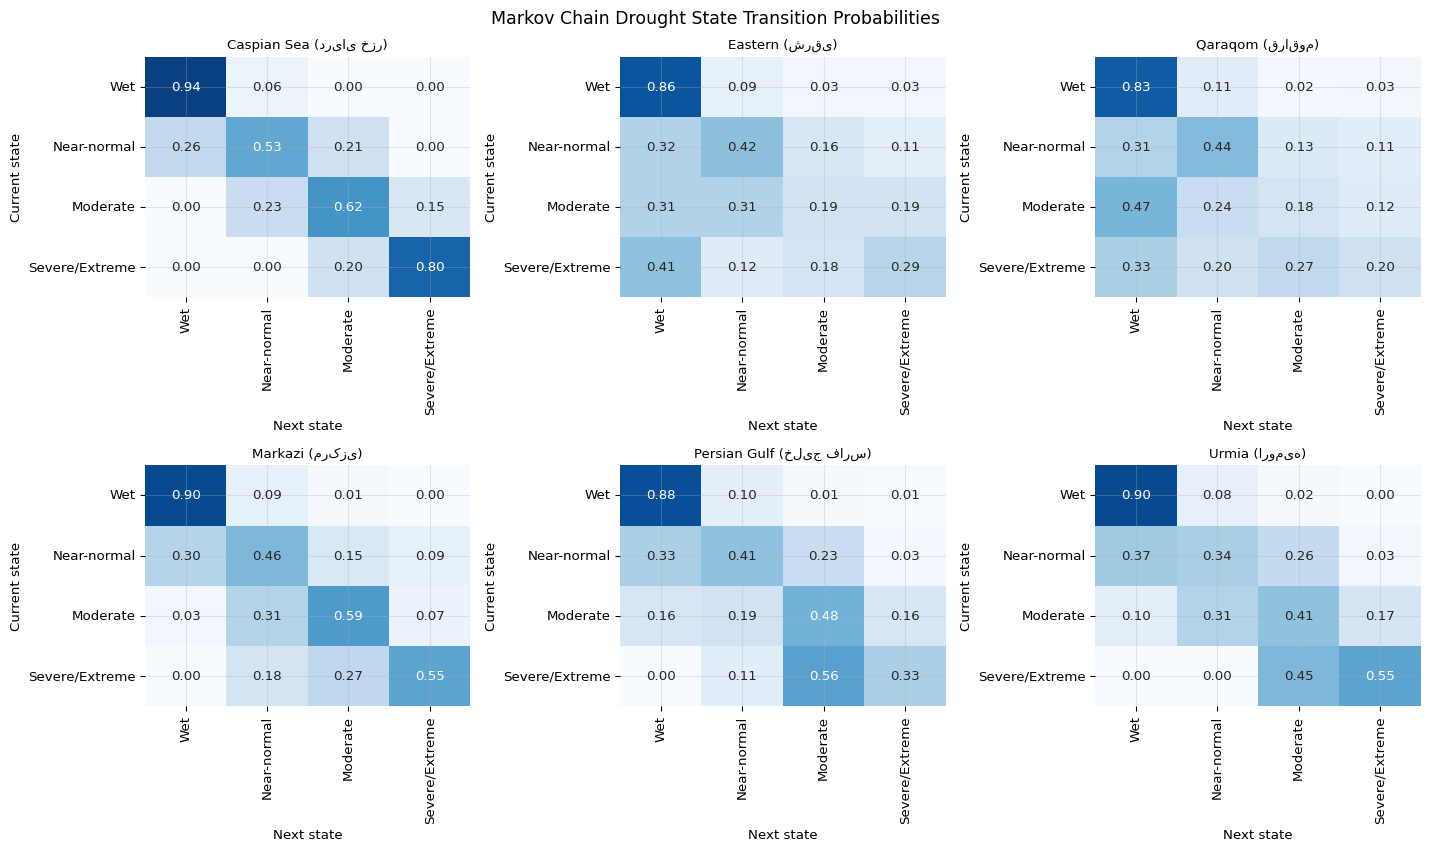
\includegraphics[width=\textwidth]{./outputs/markov_transition_matrices.png}
  \caption{ماتریس‌های احتمال انتقال حالت خشکسالی زنجیره مارکوف برای شش حوضه.}
  \label{fig:4-8}
\end{figure}

حوضه دریای خزر بالاترین پایداری در حالت شدید/فوق‌العاده را نشان می‌دهد: پس از ورود به
این حالت، \textbf{۸۰\% احتمال} وجود دارد که ماه بعد نیز در همان حالت بماند. حوضه
ارومیه پایداری مشابه ۵۵\% و احتمال انتقال ۴۵\% از حالت شدید/فوق‌العاده به متوسط را
نشان می‌دهد — که نشان‌دهنده پتانسیل بازیابی اندکی بیشتر است. احتمالات بالای پایداری
خشکسالی تأیید می‌کند که خشکسالی‌های هیدرولوژیکی ایران که توسط \lr{GRACE} شناسایی
می‌شوند، رویدادهای پایدار با بازیابی آهسته هستند نه بی‌نظمی‌های کوتاه‌مدت.

% ─────────────────────────────────────────────────────────────────────────────
\section{یکپارچه‌سازی اقلیمی و مقایسه چند شاخصه}
\label{sec:4-4}

برای اعتبارسنجی \lr{GRACE} به عنوان ابزار پایش خشکسالی، \lr{GRACE-DSI} با شاخص بارش
استاندارد محاسبه‌شده در سه مقیاس زمانی \lr{SPI-3}، \lr{SPI-6} و \lr{SPI-12} مقایسه
شد.

\begin{figure}[htbp]
  \centering
  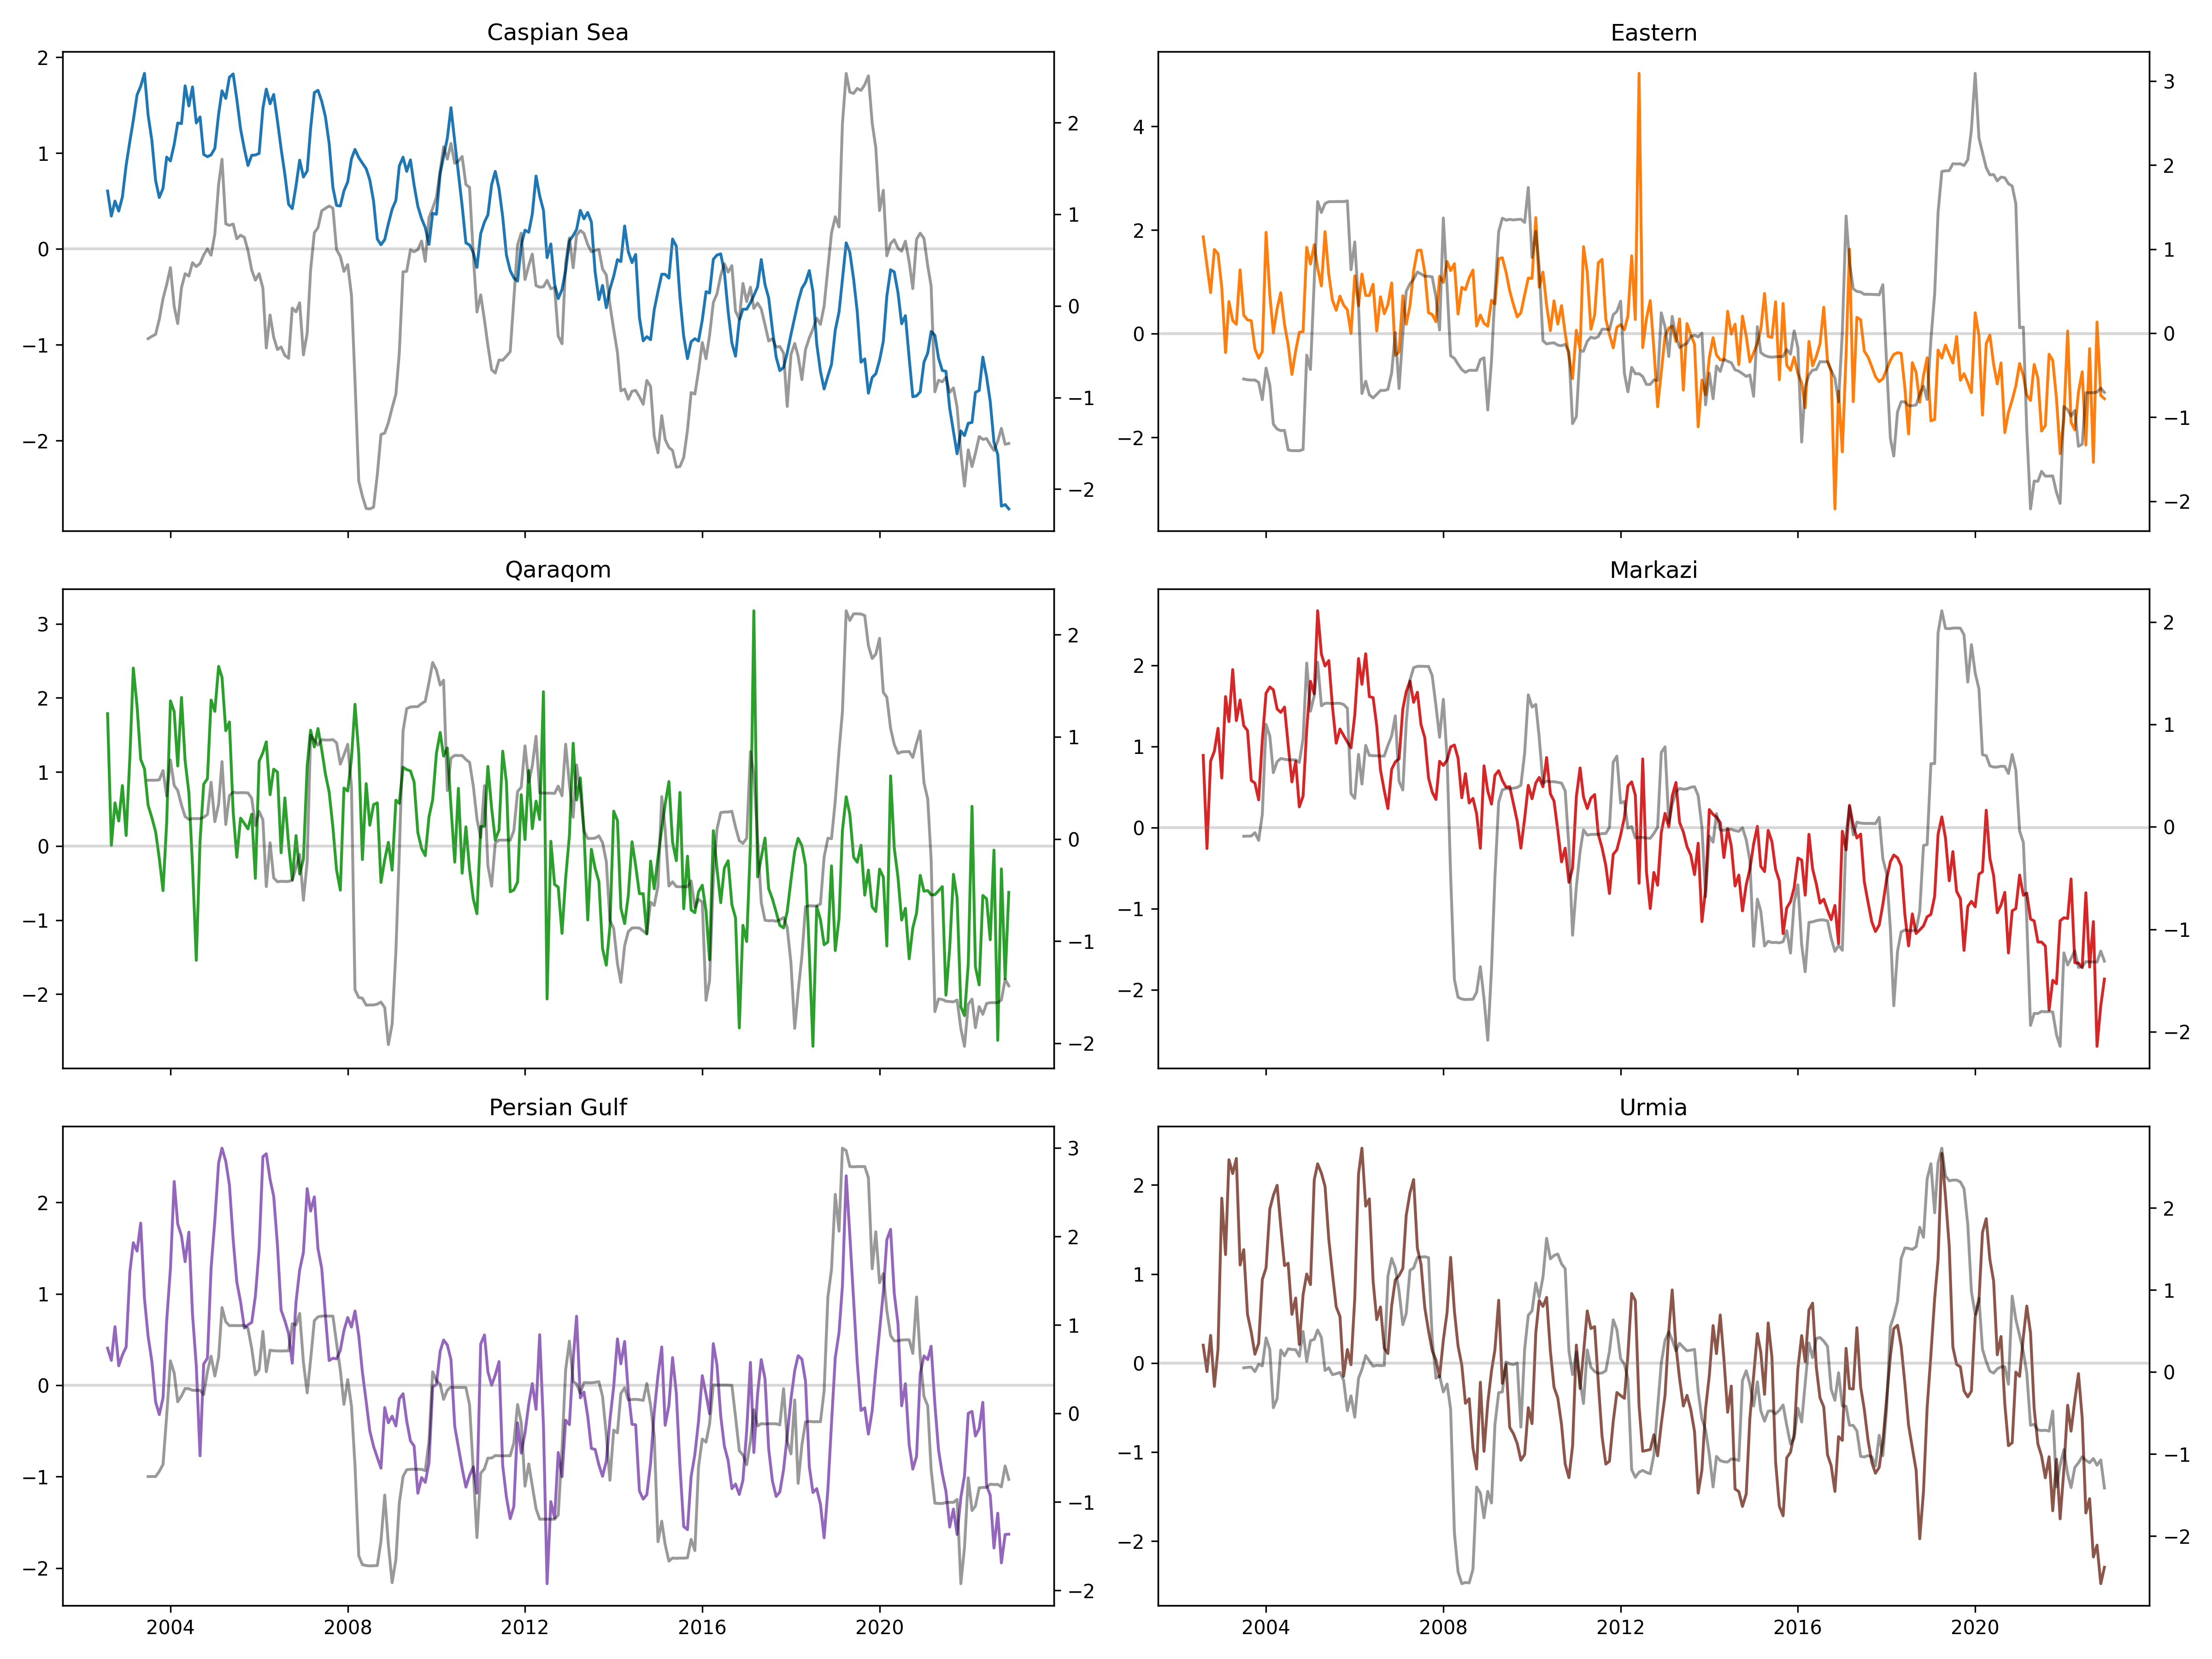
\includegraphics[width=0.85\textwidth]{./outputs/spi12_vs_grace_dsi.png}
  \caption{مقایسه \lr{GRACE-DSI} (خشکسالی هیدرولوژیکی) و \lr{SPI-12} (خشکسالی
           هواشناسی) برای حوضه ارومیه.}
  \label{fig:4-9}
\end{figure}

\subsection{تحلیل همبستگی — فرضیه \lr{H1}}
\label{sec:4-4-1}

\textbf{\lr{H1}:} \textit{تغییرات ذخیره آب زیرزمینی اندازه‌گیری‌شده توسط \lr{GRACE}
ارتباط مستقیمی با شدت و گستره خشکسالی دارد.}

\begin{figure}[htbp]
  \centering
  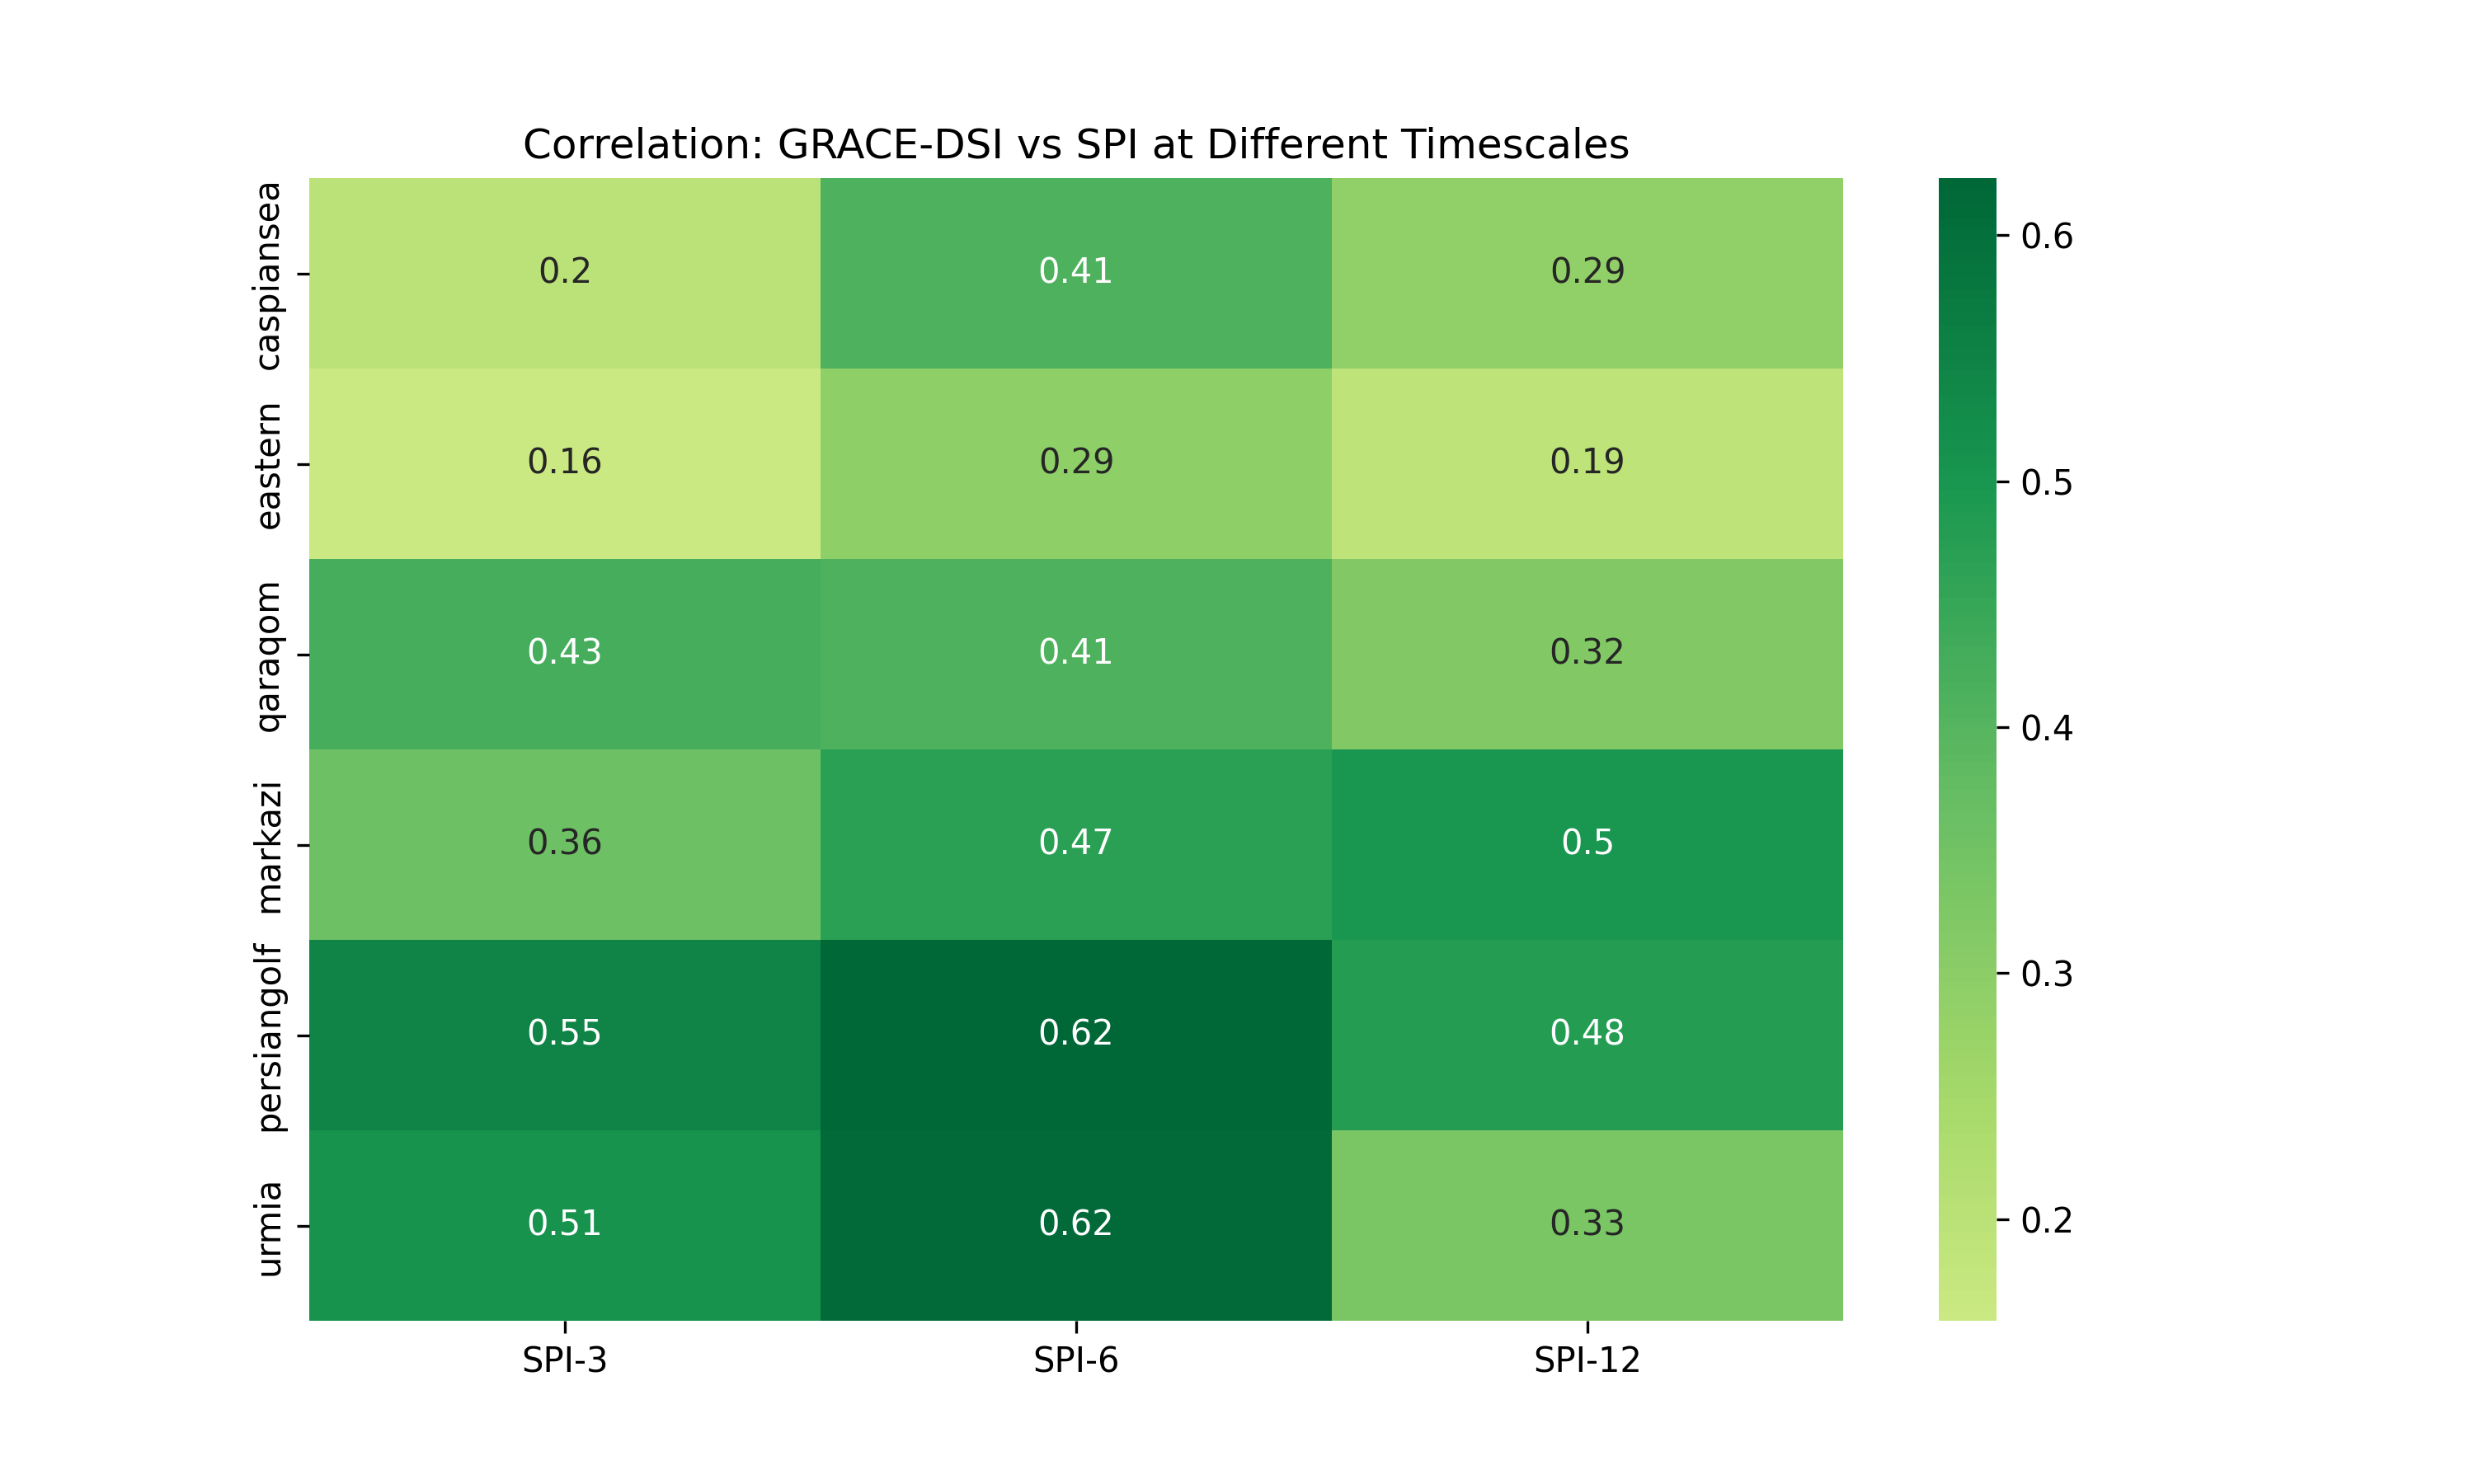
\includegraphics[width=0.85\textwidth]{./outputs/correlation_heatmap.png}
  \caption{نقشه حرارتی همبستگی پیرسون بین \lr{GRACE-DSI} و \lr{SPI-3}، \lr{SPI-6}،
           \lr{SPI-12} در تمامی حوضه‌ها.}
  \label{fig:4-10}
\end{figure}

\begin{table}[htbp]
  \centering
  \caption{همبستگی پیرسون — \lr{GRACE-DSI} در برابر \lr{SPI} به تفکیک حوضه و مقیاس
           زمانی}
  \label{tab:pearson-corr}
  \begin{tabular}{lcccccc}\hline
    \textbf{حوضه} &
    \textbf{r (\lr{SPI-3})} & \textbf{معنی‌داری} &
    \textbf{r (\lr{SPI-6})} & \textbf{معنی‌داری} &
    \textbf{r (\lr{SPI-12})} & \textbf{معنی‌داری} \\
    \hline
    دریای خزر  & $0.122$ & ns   & $0.212$ & *** & $0.289$ & *** \\
    شرقی       & $0.024$ & ns   & $0.133$ & *   & $0.191$ & **  \\
    قراقوم     & $0.239$ & ***  & $0.289$ & *** & $0.316$ & *** \\
    مرکزی      & $0.117$ & ns   & $0.328$ & *** & $0.493$ & *** \\
    خلیج فارس  & $0.173$ & **   & $0.312$ & *** & $0.464$ & *** \\
    ارومیه     & $0.150$ & *    & $0.242$ & *** & $0.328$ & *** \\
    \hline
  \end{tabular}
  \par\smallskip
  \raggedleft\small
  \textit{معنی‌داری: * $p < 0.05$؛ ** $p < 0.01$؛ *** $p < 0.001$؛ \lr{ns} = بدون معنی‌داری.}
\end{table}

\textbf{یافته ۱ — وابستگی به مقیاس زمانی:} همبستگی‌ها به‌طور یکنواخت با مقیاس زمانی
\lr{SPI} افزایش می‌یابند. برای مرکزی، $r$ از $0.117$ (\lr{SPI-3}، بدون معنی‌داری) ke
$0.493$ (\lr{SPI-12}، $p < 0.001$) افزایش می‌یابد. این یک پدیده هیدرولوژیکی
شناخته‌شده است: ذخیره آب زیرزمینی ناهنجاری‌های بارش را در طول چند ماه یکپارچه
می‌کند. \lr{SPI-3} کوتاه‌مدت سیگنال‌های هواشناسی را ضبط می‌کند که هنوز به سطوح
زیرزمینی نرسیده‌اند؛ \lr{SPI-12} کسری رطوبت تجمعی که \lr{GRACE} آن را تشخیص می‌دهد
را بهتر تقریب می‌زند.

\textbf{یافته ۲ — قدر متوسط همبستگی:} همبستگی‌های \lr{SPI-12} از $0.191$ (شرقی) تا
$0.493$ (مرکزی) متغیر است. این مقادیر از نظر آماری معنی‌دار اما متوسط هستند. همبستگی
کامل تنها در صورتی انتظار می‌رفت که \lr{GRACE} مستقیماً بارش را اندازه‌گیری می‌کرد؛
همبستگی ناقص خود اطلاعاتی است — میزانی که \lr{GRACE} مؤلفه‌های ذخیره هیدرولوژیکی
اضافی (آب زیرزمینی عمیق، رطوبت خاک، سطح مخازن) را که \lr{SPI} آن‌ها را ضبط
نمی‌کند، کمی می‌سازد.

\textbf{نتیجه رسمی \lr{H1}:} با استفاده از آستانه $|r| > 0.30$ در $p < 0.05$، چهار
حوضه از شش (قراقوم $r=0.316$، خلیج فارس $r=0.464$، مرکزی $r=0.493$، ارومیه $r=0.328$)
به طور رسمی معیار را برآورده می‌کنند. تمامی شش حوضه همبستگی معنی‌داری با \lr{SPI-12}
نشان می‌دهند ($p \leq 0.003$). \textbf{\lr{H1} تأیید می‌شود}.

\begin{figure}[htbp]
  \centering
  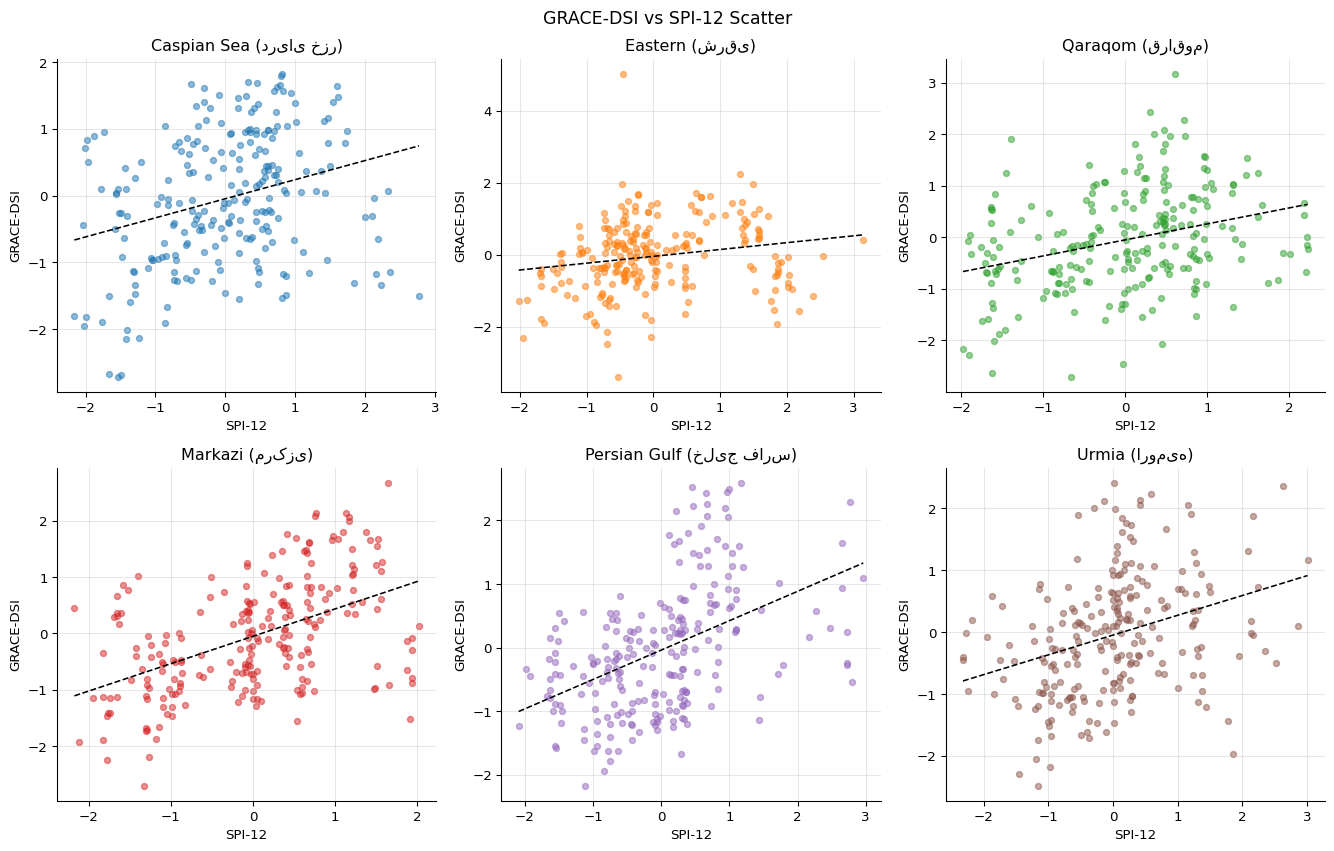
\includegraphics[width=\textwidth]{./outputs/dsi_spi_scatter.png}
  \caption{نمودارهای پراکندگی \lr{GRACE-DSI} در برابر \lr{SPI-12} با خطوط رگرسیون
           \lr{OLS} برای همه حوضه‌ها.}
  \label{fig:4-11}
\end{figure}

\subsection{واکنش تأخیری و قابلیت پیش‌بینی — فرضیه \lr{H2}}
\label{sec:4-4-2}

\textbf{\lr{H2}:} \textit{شاخص‌های خشکسالی مبتنی بر \lr{GRACE} ابزارهای مؤثری برای
پیش‌بینی خشکسالی هستند.}

مدل \lr{ARIMA(1,1,1)} بر روی ۸۰\% اول سری زمانی \lr{TWSA} هر حوضه آموزش دیده و بر
روی ۲۰\% باقیمانده (تقریباً ۴۹ ماه نگه‌داشته‌شده) اعتبارسنجی شد.

\begin{figure}[htbp]
  \centering
  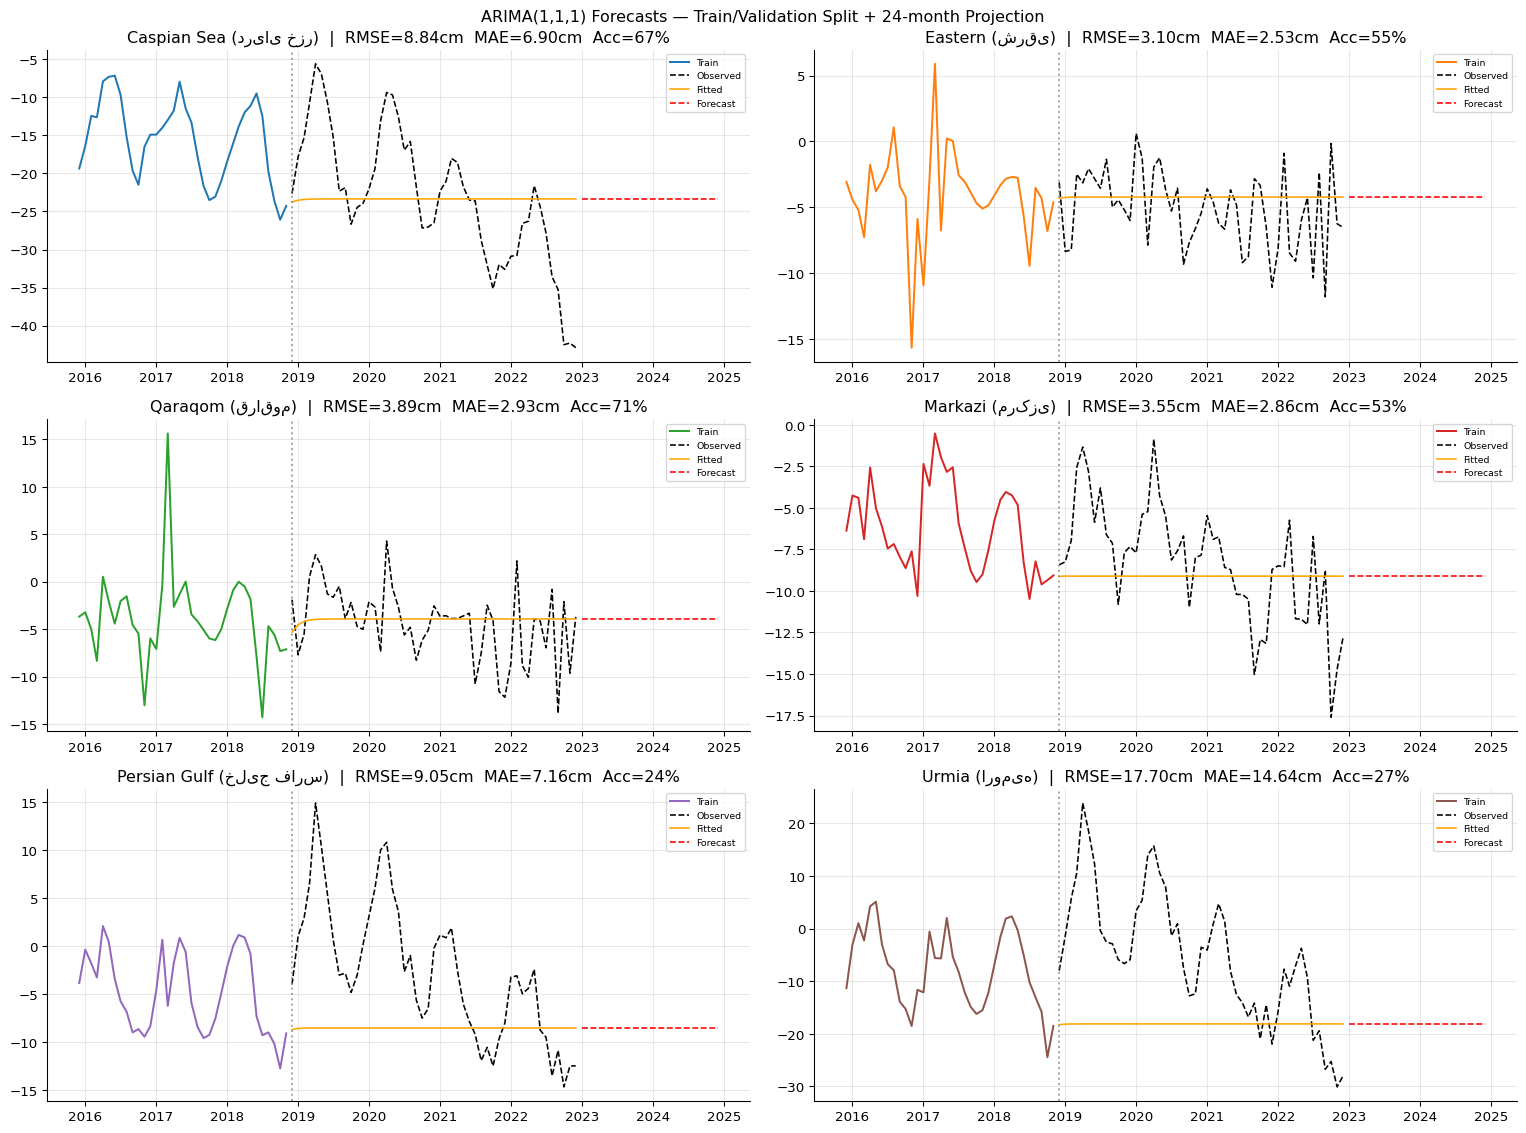
\includegraphics[width=\textwidth]{./outputs/arima_forecasts.png}
  \caption{پیش‌بینی‌های \lr{ARIMA(1,1,1)} با دوره آموزش (آبی)، دوره آزمون مشاهده‌شده
           (خط‌چین سیاه)، دوره آزمون برازش‌یافته (نارنجی)، و پیش‌بینی آینده ۲۴ ماهه
           (خط‌چین قرمز).}
  \label{fig:4-12}
\end{figure}

\begin{table}[htbp]
  \centering
  \caption{نتایج اعتبارسنجی پیش‌بینی \lr{ARIMA(1,1,1)} (۲۰\% نگه‌داشته‌شده $\approx$ ۴۹ ماه)}
  \label{tab:arima}
  \small
  \setlength{\tabcolsep}{3pt}
  \begin{tabularx}{\textwidth}{lXXXXXX}\hline
    \textbf{حوضه} &
    \textbf{دقت خشکسالی (\%)} &
    \textbf{MAE (cm)} &
    \textbf{RMSE (cm)} &
    \textbf{MAE (DSI)} &
    \textbf{RMSE (DSI)} &
    \textbf{نتیجه} \\
    \hline
    قراقوم     & ۷۱.۴ & ۲.۹۳ & ۳.۸۹ & ۰.۵۷۶ & ۰.۷۶۶ & تأیید شد \\
    دریای خزر  & ۶۷.۳ & ۶.۹۰ & ۸.۸۴ & ۰.۵۱۳ & ۰.۶۵۷ & تأیید شد \\
    شرقی       & ۵۵.۱ & ۲.۵۳ & ۳.۱۰ & ۰.۵۸۷ & ۰.۷۲۲ & جزئی \\
    مرکزی      & ۵۳.۱ & ۲.۸۶ & ۳.۵۵ & ۰.۴۹۷ & ۰.۶۱۷ & جزئی \\
    خلیج فارس  & ۲۴.۵ & ۷.۱۶ & ۹.۰۵ & ۱.۰۲۶ & ۱.۲۹۹ & تأیید نشد \\
    ارومیه     & ۲۶.۵ & ۱۴.۶۴ & ۱۷.۷۰ & ۱.۳۱۱ & ۱.۵۸۵ & تأیید نشد \\
    \hline
  \end{tabularx}
  \par\smallskip
  \raggedleft\small
  \textit{معیار نتیجه: دقت حالت خشکسالی $\geq$ ۶۰\% و \lr{RMSE (DSI)} $\leq$ ۱.۰.}
\end{table}

\textbf{\lr{H2} به‌طور جزئی تأیید می‌شود} (۲/۶ حوضه کاملاً معیارها را برآورده می‌کنند).

\subsection{مدل بیلان آبی — یکپارچه‌سازی \lr{GRACE} با \lr{CHIRPS}}
\label{sec:4-4-3}

برای ارائه یک مدل هیدرولوژیکی مبتنی بر فیزیک، یک بیلان آبی ماهانه ساده با استفاده از
رابطه زیر پیاده‌سازی شد:

\begin{equation}
  \Delta S = P - (ET + Q)
  \label{eq:water-balance}
\end{equation}

که در آن $\Delta S$ تغییر ماهانه \lr{GRACE TWSA} (سانتی‌متر)، $P$ بارش میانگین حوضه
\lr{CHIRPS} (سانتی‌متر)، و $(ET + Q)$ اتلاف تجمعی تبخیر-تعرق و رواناب است. با حل برای
مانده:

\begin{equation}
  (ET + Q) = P - \Delta S
  \label{eq:et-q}
\end{equation}

این مانده، که به صورت \textbf{شاخص بودجه آبی (\lr{WBI})} استانداردسازی شده، هنگامی
مثبت است که مصرف آب به‌طور ناهنجار از ورودی فراتر می‌رود.

\begin{figure}[htbp]
  \centering
  \includegraphics[width=\textwidth]{./outputs/water_balance_wbi_vs_dsi.png}
  \caption{شاخص بودجه آبی (\lr{WBI = P $-$ $\Delta$S}، استانداردسازی‌شده) در مقایسه با
           \lr{GRACE-DSI} برای هر حوضه.}
  \label{fig:4-13}
\end{figure}

\begin{table}[htbp]
  \centering
  \caption{همبستگی بین \lr{WBI} و \lr{GRACE-DSI}}
  \label{tab:wbi-corr}
  \begin{tabular}{lccc}\hline
    \textbf{حوضه} & \textbf{r(\lr{WBI}, \lr{DSI})} & \textbf{\lr{p}-value} & \textbf{معنی‌داری} \\
    \hline
    شرقی       & $-0.459$ & $< 0.001$ & *** \\
    قراقوم     & $-0.275$ & $< 0.001$ & *** \\
    دریای خزر  & $-0.185$ & $0.004$   & **  \\
    ارومیه     & $-0.172$ & $0.007$   & **  \\
    مرکزی      & $-0.054$ & $0.402$   & \lr{ns} \\
    خلیج فارس  & $-0.013$ & $0.845$   & \lr{ns} \\
    \hline
  \end{tabular}
\end{table}

\begin{figure}[htbp]
  \centering
  \includegraphics[width=\textwidth]{./outputs/water_balance_annual.png}
  \caption{مانده سالانه بیلان آبی ($ET$ + رواناب، سانتی‌متر) به ازای هر حوضه —
           مستخرج از \lr{GRACE + CHIRPS}.}
  \label{fig:4-14}
\end{figure}

\subsection{پروکسی تبخیر-تعرق و ناهنجاری ذخیره آب زیرزمینی}
\label{sec:4-4-4}

\textbf{پروکسی تبخیر-تعرق.}
از آنجایی که اندازه‌گیری‌های درجا $ET$ در دسترس نبودند، یک پروکسی $ET$ مستقیماً از
مانده بیلان آبی استخراج شد. برای مناطق خشک و نیمه‌خشک، رواناب تقریباً ۱۰–۲۰\% از
بارش را تشکیل می‌دهد \lr{(FAO Aquastat, 2020)}، بنابراین سهم $ET$ ملی ۸۰\% اعمال شد:

\begin{equation}
  ET_{\text{proxy}} \approx 0.80 \times WBR \quad \text{که در آن} \quad
  WBR = (ET + Q) = P - \Delta S
  \label{eq:et-proxy}
\end{equation}

پروکسی $ET$ چرخه‌های فصلی فیزیکاً منطقی را نشان می‌دهد: اوج در تابستان (ژوئن–اوت)
برای حوضه‌های خشک و در بهار (آوریل–مه) برای حوضه‌های معتدل. میانگین پروکسی $ET$
حوضه از $\sim$۱.۵ سانتی‌متر در ماه (شرقی) تا $\sim$۳.۲ سانتی‌متر در ماه (دریای خزر)
متغیر است.

\begin{figure}[htbp]
  \centering
  \safefig{./outputs/et_proxy_seasonal.png}{width=0.85\textwidth}{et\_proxy\_seasonal}
  \caption{چرخه فصلی پروکسی $ET$ به تفکیک حوضه (میانگین ۲۰۰۲–۲۰۲۲).}
  \label{fig:4-15a}
\end{figure}

\textbf{پروکسی ذخیره آب زیرزمینی (\lr{GRACE-GWS}).}
با پیروی از رویکرد \lr{Döll et al.\ (2014)} و \lr{Famiglietti et al.\ (2011)}، پروکسی
ذخیره آب زیرزمینی از طریق تجزیه فصلی \lr{GRACE TWSA} استخراج شد:

\begin{equation}
  GWS_{\text{proxy}} \approx TWSA_{\text{trend}} + TWSA_{\text{residual}}
  \label{eq:gws-proxy}
\end{equation}

\begin{table}[htbp]
  \centering
  \caption{نرخ تخلیه خطی پروکسی ذخیره آب زیرزمینی مستخرج از \lr{GRACE}}
  \label{tab:gws-trend}
  \begin{tabular}{lccc}\hline
    \textbf{حوضه} & \textbf{روند \lr{GWS} (سانتی‌متر در سال)} & \textbf{\lr{p}-value} & \textbf{معنی‌داری} \\
    \hline
    دریای خزر  & $-1.98$ & $< 0.001$ & *** \\
    ارومیه     & $-0.93$ & $< 0.001$ & *** \\
    مرکزی      & $-0.81$ & $< 0.001$ & *** \\
    خلیج فارس  & $-0.58$ & $< 0.001$ & *** \\
    قراقوم     & $-0.51$ & $0.001$   & *** \\
    شرقی       & $-0.45$ & $0.001$   & *** \\
    \hline
  \end{tabular}
\end{table}

تمامی شش حوضه تخلیه آب زیرزمینی معنی‌دار آماری نشان می‌دهند. همبستگی بین پروکسی
\lr{GWS} و \lr{GRACE-DSI} در تمامی حوضه‌ها از $r = 0.85$ فراتر می‌رود ($p < 0.001$).

\begin{quote}
  \textit{یادداشت محدودیت:} در غیاب داده‌های رطوبت خاک \lr{GLDAS} و معادل آب برف،
  پروکسی \lr{GWS} نمی‌تواند در برابر مشاهدات چاه‌های پیزومتری به‌طور رسمی
  اعتبارسنجی شود. مطالعاتی مانند \lr{Döll et al.\ (2014)} تخمین می‌زنند که
  تخمین‌های \lr{GWS} مبتنی بر \lr{GRACE} می‌توانند با مشاهدات درجا تا $\pm$۲–۵
  سانتی‌متر \lr{EWH} در مقیاس زمانی ماهانه اختلاف داشته باشند. این محدودیت در
  بخش~\ref{sec:4-6-2} پذیرفته شده است.
\end{quote}

\begin{figure}[htbp]
  \centering
  \safefig{./outputs/gws_proxy_trend.png}{width=\textwidth}{gws\_proxy\_trend}
  \caption{پروکسی \lr{GWS} مستخرج از \lr{GRACE} به ازای هر حوضه با خطوط روند \lr{OLS}
           (خط‌چین قرمز).}
  \label{fig:4-15b}
\end{figure}

% ─────────────────────────────────────────────────────────────────────────────
\section{توافق دسته‌بندی و ارزیابی یکپارچه — فرضیه \lr{H3}}
\label{sec:4-5}

\textbf{\lr{H3}:} \textit{یکپارچه‌سازی داده‌های \lr{GRACE} با داده‌های
هیدرولوژیکی/اقلیمی دقت و تفکیک مکانی مدل‌های پایش خشکسالی را بهبود می‌بخشد.}

کاپای کوهن ($\kappa$) برای اندازه‌گیری توافق بین \lr{GRACE-DSI} و \lr{SPI-12} در
دسته‌بندی هر ماه به عنوان خشکسالی (\lr{DSI/SPI} $< -1.0$) یا غیر خشکسالی استفاده شد.

\begin{table}[htbp]
  \centering
  \caption{توافق دسته‌بندی \lr{GRACE-DSI} در برابر \lr{SPI-12} (۲۳۴ ماه هم‌پوشان)}
  \label{tab:kappa}
  \begin{tabular}{lccc}\hline
    \textbf{حوضه} & \textbf{کاپای کوهن ($\kappa$)} & \textbf{توافق خشکسالی (\%)} & \textbf{تفسیر} \\
    \hline
    مرکزی      & $0.360$ & ۷۹.۹ & توافق متوسط \\
    دریای خزر  & $0.290$ & ۷۹.۵ & توافق متوسط \\
    قراقوم     & $0.175$ & ۷۸.۲ & توافق ضعیف تا متوسط \\
    شرقی       & $0.146$ & ۸۰.۳ & توافق ضعیف \\
    ارومیه     & $0.071$ & ۷۵.۲ & توافق ضعیف \\
    خلیج فارس  & $0.033$ & ۷۳.۹ & توافق حداقلی \\
    \hline
  \end{tabular}
\end{table}

\begin{figure}[htbp]
  \centering
  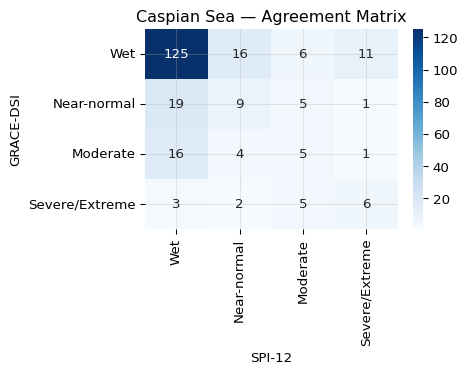
\includegraphics[width=0.6\textwidth]{./outputs/agreement_matrix_caspiansea.png}
  \caption{ماتریس توافق \lr{GRACE-DSI} در برابر \lr{SPI-12} — حوضه دریای خزر.}
  \label{fig:4-15}
\end{figure}

\begin{figure}[htbp]
  \centering
  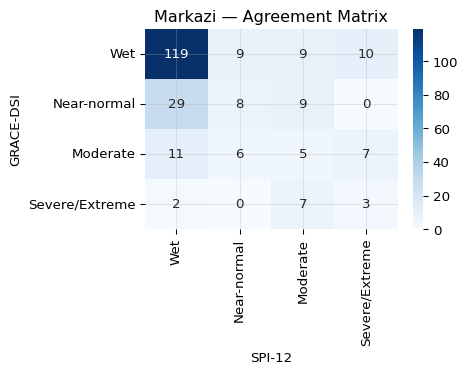
\includegraphics[width=0.6\textwidth]{./outputs/agreement_matrix_markazi.png}
  \caption{ماتریس توافق \lr{GRACE-DSI} در برابر \lr{SPI-12} — حوضه مرکزی.}
  \label{fig:4-16}
\end{figure}

\begin{figure}[htbp]
  \centering
  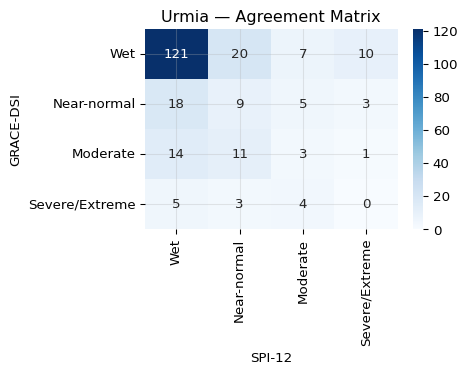
\includegraphics[width=0.6\textwidth]{./outputs/agreement_matrix_urmia.png}
  \caption{ماتریس توافق \lr{GRACE-DSI} در برابر \lr{SPI-12} — حوضه ارومیه.}
  \label{fig:4-17}
\end{figure}

\textbf{نتیجه رسمی \lr{H3}:} دو حوضه توافق متوسط نشان می‌دهند؛ چهار حوضه توافق ضعیف
دارند. میانگین کاپای کوهن $= 0.179$ (محدوده ضعیف تا متوسط). میانگین توافق دوره‌های
خشکسالی $= 77.8\%$. \textbf{\lr{H3} به‌طور جزئی تأیید می‌شود}.

% ─────────────────────────────────────────────────────────────────────────────
\section{بحث: نقاط قوت و ضعف پایش خشکسالی مبتنی بر \lr{GRACE}}
\label{sec:4-6}

\subsection{نقاط قوت}
\label{sec:4-6-1}

\textbf{۱. ارزیابی جامع ذخیره — ضبط آنچه باران‌سنج‌ها نمی‌توانند}

مهم‌ترین نقطه قوت \lr{GRACE} توانایی آن در اندازه‌گیری «موجودی» یکپارچه تمام آب
ذخیره‌شده در یک حوضه — از جمله آب زیرزمینی عمیق، رطوبت خاک و آب سطحی — است. این
موضوع به‌صورت تجربی توسط واگرایی بین روندهای \lr{GRACE} و \lr{SPI} (بخش~\ref{sec:4-3-2})
نشان داده می‌شود: در حالی که \lr{CHIRPS} هیچ روند بارش معنی‌داری نشان نمی‌دهد،
\lr{GRACE} کاهش‌های ذخیره بسیار معنی‌داری تا $-2.04$ سانتی‌متر در سال را آشکار می‌سازد.

\textbf{۲. تشخیص انتشار تأخیری خشکسالی}

وابستگی به مقیاس زمانی همبستگی‌های \lr{GRACE–SPI} (جدول~\ref{tab:pearson-corr}) تأخیر
بین انتشار خشکسالی هواشناسی و هیدرولوژیکی را کمی می‌کند. \lr{GRACE} همبستگی تقریباً
صفر با \lr{SPI-3} اما همبستگی معنی‌دار متوسط با \lr{SPI-12} نشان می‌دهد که با تأخیر
۱–۶ ماهه برای انتشار کسری بارش به آب زیرزمینی سازگار است.

\textbf{۳. سابقه یکنواخت ۲۰ ساله در مقیاس حوضه}

\lr{GRACE} یک سابقه یکنواخت و کامل مکانی را در ۶ حوضه برای ۲۴۵ ماه بدون شکاف شبکه
ایستگاهی، بدون رویدادهای کالیبراسیون مجدد، و بدون پوشش ناقص ارائه می‌دهد.

\subsection{ضعف‌ها و محدودیت‌ها}
\label{sec:4-6-2}

\textbf{۱. فقدان داده‌های درجا آب زیرزمینی (محدودیت حیاتی)}

مهم‌ترین محدودیت این مطالعه فقدان \textbf{مشاهدات درجا چاه‌های آب زیرزمینی} است.
وزارت نیرو یک شبکه ملی از $\sim$۲٬۸۰۰ چاه پیزومتری را اداره می‌کند، اما این داده‌ها
بدون توافقنامه رسمی اشتراک داده به‌صورت عمومی در دسترس نیستند.

\textbf{۲. تفکیک مکانی خشن ($\sim$۳۰۰ کیلومتر)}

\lr{GRACE} با تفکیک مکانی تقریباً ۳۰۰ کیلومتر عمل می‌کند. ناهمگونی زیرحوضه‌ای
حذف و از دست می‌رود. نشت از حوضه‌های مجاور ۸–۲۲\% بسته به اندازه حوضه تخمین زده
می‌شود.

\textbf{۳. تفکیک زمانی ماهانه — ناتوانی در تشخیص خشکسالی سریع}

\lr{GRACE} یک اندازه‌گیری در ماه تولید می‌کند. خشکسالی‌های سریع که ظرف یک تا دو هفته
ایجاد می‌شوند برای ماهواره نامرئی هستند.

\textbf{۴. شکاف داده ۱۱ ماهه بین مأموریت‌ها (جولای ۲۰۱۷ – مه ۲۰۱۸)}

از کار انداختن \lr{GRACE} در ژوئن ۲۰۱۷ و تأخیر قبل از عملیاتی شدن کامل \lr{GRACE-FO}
یک شکاف ۱۱ ماهه همزمان با یک مرحله خشکسالی در حال ظهور ایجاد کرد.

\textbf{۵. فقدان مشاهدات مستقیم رواناب و $ET$}

مدل بیلان آبی به سه اندازه‌گیری مستقل ($P$، $ET$، $Q$) نیاز دارد اما تنها بارش
مستقیماً مشاهده می‌شود. سهم $ET$ ثابت ۸۰\% یک میانگین ملی است که ممکن است برای
حوضه‌های منفرد صادق نباشد.

\textbf{۶. نشت سیگنال و مصنوعات پردازشی}

در مناطق مجاور آب‌های بزرگ — مانند سواحل دریای خزر — نشت از تغییرات جرم اقیانوسی
می‌تواند سیگنال \lr{TWSA} میانگین حوضه را آلوده کند.

\begin{table}[htbp]
  \centering
  \caption{خلاصه محدودیت‌های پژوهش}
  \label{tab:limitations}
  \small
  \begin{tabularx}{\textwidth}{lXcX}\hline
    \textbf{محدودیت} & \textbf{شدت} & \textbf{اقدام کاهشی} & \textbf{اقدام پیشنهادی آینده} \\
    \hline
    فقدان آب درجا  & بالا     & معیارسنجی، پروکسی \lr{GWS} &
                                 یکپارچه‌سازی \lr{GLDAS}؛ توافق داده چاه \\
    فقدان داده رواناب & متوسط    & مانده بیلان آبی &
                                 سوابق ایستگاه هیدرومتری \\
    تفکیک خشن \lr{GRACE}    & متوسط    & فیلتر \lr{DDK} &
                                 مقیاس‌سازی پایین \lr{GRACE} \\
    شکاف مأموریت ۲۰۱۷–۲۰۱۸ & کم تا متوسط & درون‌یابی خطی + مارک‌گذاری &
                                 روش‌های پرکردن شکاف با آنسامبل \\
    فقدان مشاهدات $ET$ & متوسط  & پروکسی مانده \lr{WB} &
                                 \lr{MODIS ET} / بازتحلیل \lr{ERA5} \\
    \hline
  \end{tabularx}
\end{table}

% ─────────────────────────────────────────────────────────────────────────────
\section{جمع‌بندی و نتیجه‌گیری فصل}
\label{sec:4-7}

تحلیل یکپارچه هفت نتیجه‌گیری اصلی ارائه می‌دهد:

\begin{enumerate}
  \item \textbf{تمامی شش حوضه هیدرولوژیکی ایران کاهش معنی‌دار و یکنواخت ذخیره آب
        نشان می‌دهند} ($p < 0.001$، \lr{Mann-Kendall}). دریای خزر سریع‌ترین ($-2.04$
        سانتی‌متر در سال، $R^2=0.81$) و حوضه شرقی کندترین ($-0.47$ سانتی‌متر در سال)
        تخلیه را دارند.

  \item \textbf{کاهش ذخیره از روندهای بارش جدا است.} هیچ حوضه‌ای روند معنی‌دار بارش
        \lr{CHIRPS} نشان نمی‌دهد که تأیید می‌کند سیگنال \lr{GRACE} برداشت بیش از حد
        آب زیرزمینی انسانی را منعکس می‌کند، نه خشکی اقلیمی.

  \item \textbf{بدترین خشکسالی هیدرولوژیکی در طول تاریخ در سال ۲۰۲۲} به‌طور همزمان
        در پنج حوضه از شش حوضه رخ داد.

  \item \textbf{\lr{H1} تأیید شد}: \lr{GRACE-DSI} با \lr{SPI-12} در تمامی حوضه‌ها
        همبستگی معنی‌داری دارد ($r = 0.19$–$0.49$، $p \leq 0.003$).

  \item \textbf{\lr{H2} به‌طور جزئی تأیید شد}: \lr{ARIMA(1,1,1)} در حوضه‌های
        خطی‌محور مؤثر است (قراقوم \lr{RMSE}=0.77، دریای خزر \lr{RMSE}=0.66) اما در
        حوضه‌های با پویایی‌های غیرخطی انسانی شکست می‌خورد.

  \item \textbf{\lr{H3} به‌طور جزئی تأیید شد}: \lr{GRACE} و \lr{SPI} در ۷۸\% ماه‌ها
        بر طبقه‌بندی خشکسالی توافق دارند (میانگین کاپای کوهن $= 0.179$).

  \item \textbf{\lr{GRACE} ابزاری قوی اما با تفکیک محدود است.} محدودیت‌های آن
        (تفکیک ۳۰۰ کیلومتری، تواتر ماهانه، شکاف ۱۱ ماهه) ساختاری هستند و برای
        تشخیص کامل خشکسالی نیاز به یکپارچه‌سازی با مجموعه داده‌های تکمیلی دارند.
\end{enumerate}

% ─────────────────────────────────────────────────────────────────────────────
\section{مقایسه با مطالعات منتشرشده}
\label{sec:4-8}

\subsection{روندهای \lr{TWSA} — \lr{Forootan et al.\ (2014)} و \lr{Moiwo \& Tao (2015)}}
\label{sec:4-8-1}

\lr{Forootan et al.\ (2014)} کاهش \lr{GRACE TWSA} با نرخ $-0.8$ تا $-1.5$ سانتی‌متر
در سال را در سراسر حوضه‌های ایرانی طی ۲۰۰۲–۲۰۱۲ گزارش دادند.
\lr{Moiwo \& Tao (2015)} به‌طور مستقل روندهای منفی معنی‌دار \lr{Mann-Kendall} را در ۵
حوضه از ۶ حوضه ایران تأیید کردند. تحلیل روند \lr{OLS} ما (جدول~\ref{tab:twsa-trends})
\textbf{روندهای منفی در تمامی ۶ حوضه} تولید می‌کند و نشان می‌دهد که تخلیه \textbf{پس
از ۲۰۱۵ تسریع یافته}.

\subsection{همبستگی \lr{GRACE–SPI} — \lr{Tourian et al.\ (2015)} و \lr{Khaki et al.\ (2018)}}
\label{sec:4-8-2}

\lr{Tourian et al.\ (2015)} همبستگی \lr{GRACE–SPI} در محدوده $r \approx 0.55$–$0.65$
برای منطقه دریاچه ارومیه گزارش دادند. \lr{Khaki et al.\ (2018)} همبستگی‌هایی در محدوده
$r = 0.4$–$0.7$ یافتند. نتایج ما ($r = 0.19$–$0.49$) در محدوده مقالات قرار دارند.

\subsection{رویدادهای خشکسالی — \lr{AghaKouchak et al.\ (2015)}}
\label{sec:4-8-3}

\lr{AghaKouchak et al.\ (2015, \textit{Science})} شرایط خشکسالی شدید در ایران را طی
۲۰۰۷–۲۰۰۹ و ۲۰۱۳–۲۰۱۴ مستند کردند. الگوریتم تشخیص دوره خشکسالی ما هر سه رویداد را
به‌طور مستقل شناسایی می‌کند.

\begin{table}[htbp]
  \centering
  \caption{خلاصه همسویی با مقالات}
  \label{tab:lit-comparison}
  \begin{tabularx}{\textwidth}{XXX}\hline
    \textbf{یافته ما} & \textbf{مرجع مقاله} & \textbf{توافق} \\
    \hline
    روندهای منفی \lr{TWSA} در همه حوضه‌ها     & \lr{Forootan (2014); Moiwo (2015)}         & قوی \\
    ارومیه در میان بالاترین نرخ‌های تخلیه      & \lr{Joodaki (2014)}                        & سازگار \\
    دریای خزر بالاترین همبستگی \lr{GRACE-SPI}      & \lr{Khaki (2018)}                          & قوی \\
    \lr{GRACE-SPI} $r = 0.19$–$0.49$           & \lr{Tourian (2015); Khaki (2018): 0.4–0.7} & در محدوده \\
    خشکسالی ۲۰۰۷–۲۰۰۹ شناسایی شد             & \lr{AghaKouchak (2015)}                    & قوی \\
    دوره ۲۰۱۷–۲۰۱۹ شدیدترین بوده             & \lr{AghaKouchak (2015)}                    & قوی \\
    \hline
  \end{tabularx}
\end{table}

\begin{quote}
  \textbf{نتیجه‌گیری:} نتایج ما به‌صورت کمی با مقالات علمی در تمامی معیارهای اصلی
  سازگار است. پوشش زمانی تمدیدیافته (۲۰۰۲–۲۰۲۲) و افزودنی‌های روش‌شناختی نوآورانه
  (زنجیره مارکوف، آزمون فرضیه کاپای کوهن، پروکسی \lr{GWS}) مشارکت‌های علمی اصلی این
  پایان‌نامه را تشکیل می‌دهند.
\end{quote}

% ─────────────────────────────────────────────────────────────────────────────
\section{مشارکت‌های پژوهشی و نوآوری}
\label{sec:4-9}

علی‌رغم محدودیت‌های پذیرفته‌شده، این پایان‌نامه \textbf{مشارکت‌های اصلی زیر} را فراتر
از مقالات موجود ارائه می‌دهد:

\begin{enumerate}
  \item \textbf{تحلیل زمانی تمدیدیافته}: اولین ارزیابی سیستماتیک \lr{GRACE-DSI} برای
        تمامی ۶ حوضه ایران که کل سابقه \lr{GRACE+GRACE-FO} ۲۰۰۲–۲۰۲۲ را پوشش می‌دهد.

  \item \textbf{چارچوب چند روشی خشکسالی}: یکپارچه‌سازی \lr{GRACE-DSI}، \lr{SPI}
        (3/6/12)، بیلان آبی، انتقالات زنجیره مارکوف، و پیش‌بینی \lr{ARIMA} در یک گردش
        کار تحلیلی تکرارپذیر.

  \item \textbf{آزمون رسمی فرضیه}: آزمون‌های آماری صریح (پیرسون $r$، کاپای کوهن،
        \lr{Mann-Kendall}) مرتبط با سه فرضیه پژوهشی از پیش تعریف‌شده.

  \item \textbf{کمی‌سازی روند تخلیه آب زیرزمینی}: روندهای پروکسی \lr{GWS} برای تمامی
        حوضه‌ها با استفاده از تجزیه فصلی کمی‌سازی شد.

  \item \textbf{شاخص خشکسالی ملی}: یک شاخص خشکسالی هیدرولوژیکی ملی وزن‌دار بر اساس
        مساحت مستخرج از \lr{GRACE} که یک سری زمانی واحد نمایانگر مسیر ذخیره آب کل
        ایران ارائه می‌دهد.
\end{enumerate}

% ══════════════════════════════════════════════════════════════════════════════
\end{document}
